\chapter{Prezentacja warstwy użytkowej projektu}
\label{chap:Prezentacja warstwy użytkowej projektu}
Cały projekt znajduje się na moim repozytorium: \url{https://github.com/MarcinKida/ProjektJava/tree/master}
Baza danych do tego projektu jest zamieszczona w README.md 
Użytkownik utworzony w bazie danych ma login admin, natomiast jego hasło to admin1
\section{MenuGlowne}
\label{sec:MenuGlowne}
Pierwsze rzeczą jaka ukaże się użytkownikowi po uruchomieniu programu jest MenuGlowne. Jest ono przedstawione na rysunku poniżej.
\begin{figure}[H]
    \centering
    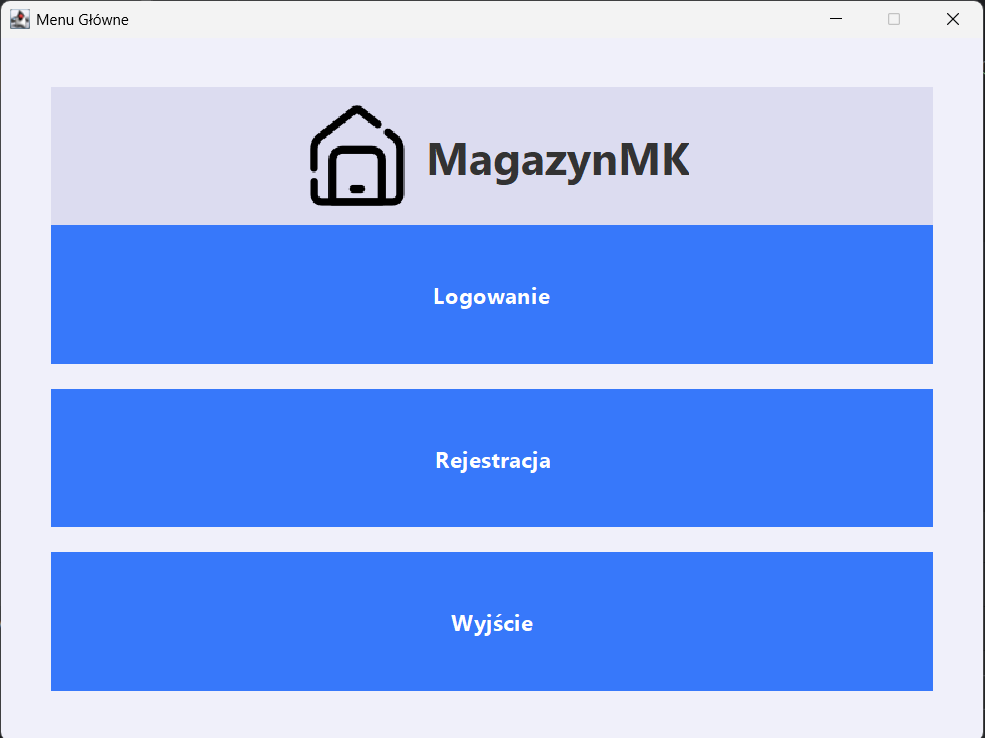
\includegraphics[width=.7\linewidth]{figures/MenuGlowne.png}\
    \caption{MenuGlowne.\label{MenuGlowne}}
\end{figure}
\clearpage
Po kliknięciu przycisku Wyjscie GUI się wyłącza. Natomiast po kliknięciu Zarejestruj przenosi nas do OknoRejestracji
\section{OknoRejestracji}
\label{sec:OknoRejestracji}

Tak wygląda okno rejestracji
\begin{figure}[H]
    \centering
    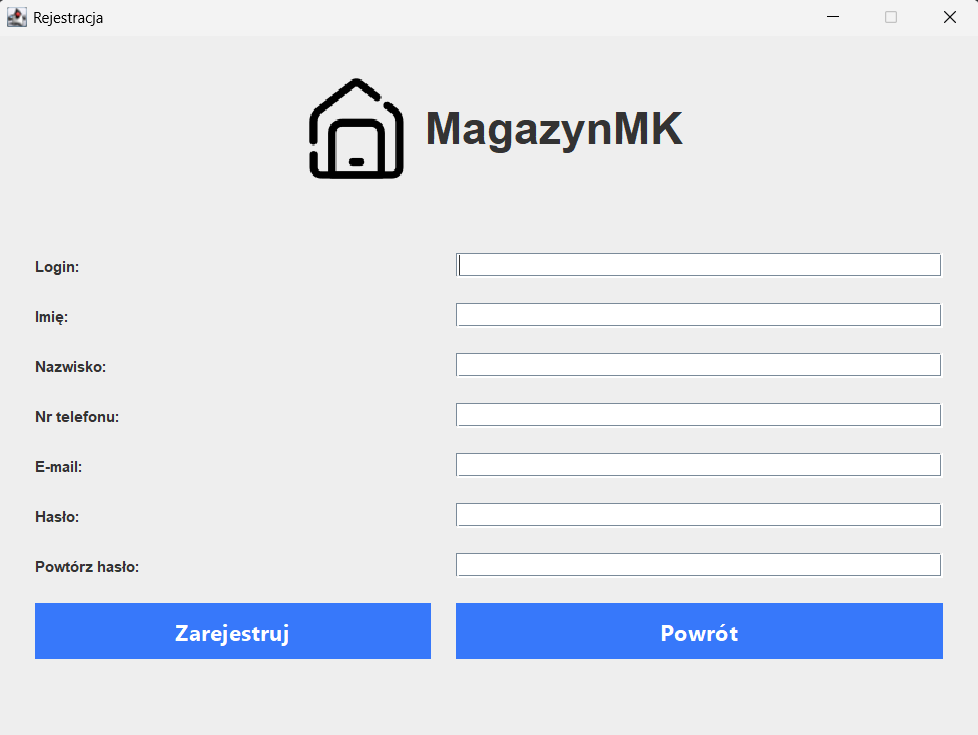
\includegraphics[width=.7\linewidth]{figures/OknoRejestracji.png}\
    \caption{OknoRejestracji.\label{OknoRejestracji}}
\end{figure}
Jeśli login ma mniej niż 4 litery lub cyfry wyskakuje taki komunikat:
\begin{figure}[H]
    \centering
    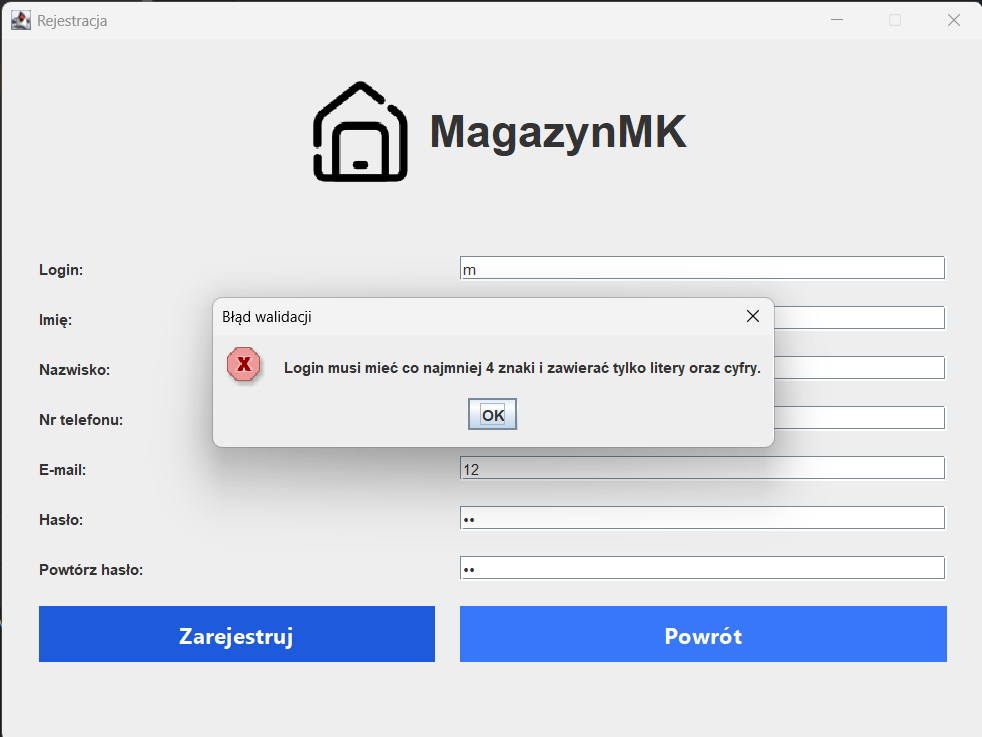
\includegraphics[width=.7\linewidth]{figures/RejestracjaKom1.png}\
    \caption{Komunikat1.\label{Komunikat1}}
\end{figure}
Jeśli Nr.Tel nie ma od 9 do 11 cyfr wyrzuca taki komunikat:
\begin{figure}[H]
    \centering
    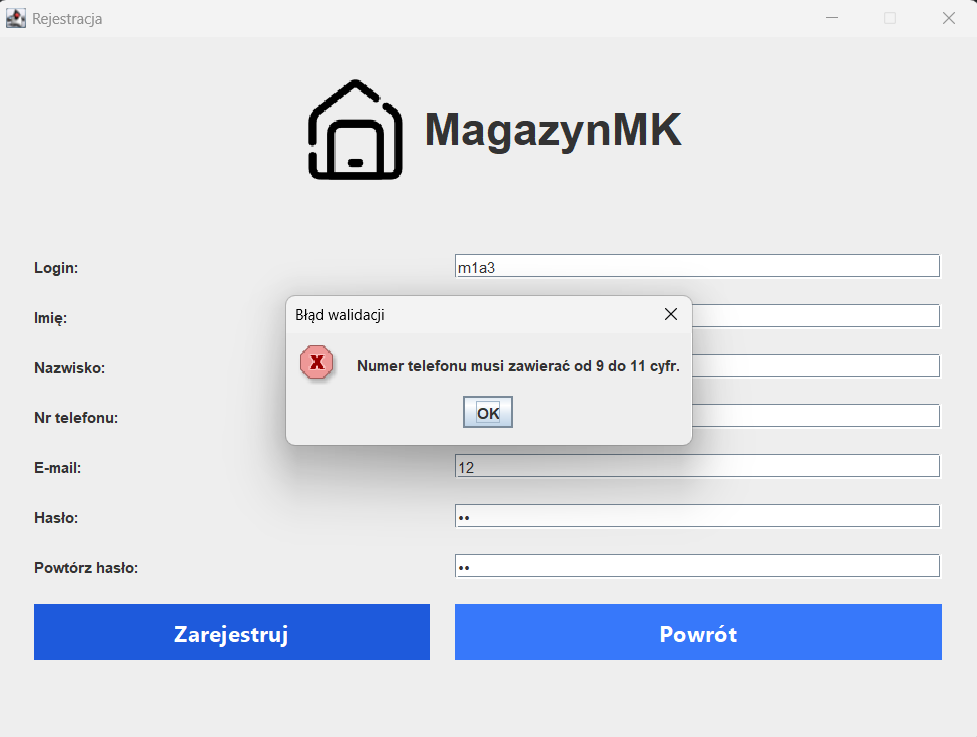
\includegraphics[width=.7\linewidth]{figures/RejestracjaKom2.png}\
    \caption{Komunikat2.\label{Komunikat2}}
\end{figure}
Jeśli email nie ma w sobie "@" wyrzuca taki komunikat:
\begin{figure}[H]
    \centering
    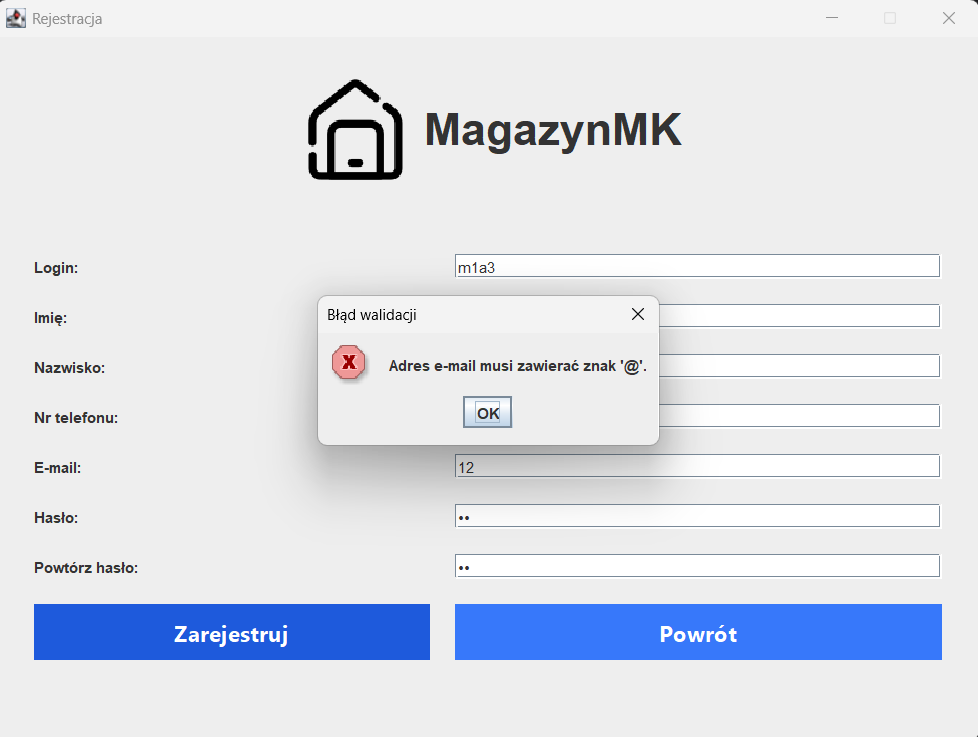
\includegraphics[width=.7\linewidth]{figures/RejestracjaKom3.png}\
    \caption{Komunikat3.\label{Komunikat3}}
\end{figure}
Jeśli hasła się nie pokrywają wyświetla taki komunikat:
\begin{figure}[H]
    \centering
    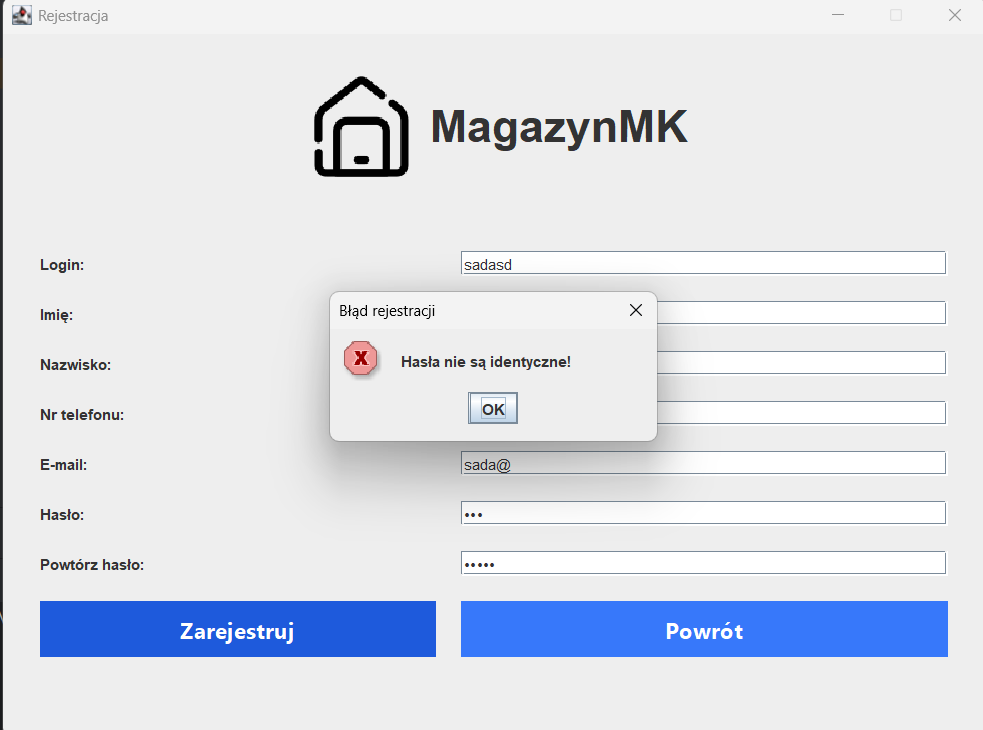
\includegraphics[width=.7\linewidth]{figures/RejestracjaKom4.png}\
    \caption{Komunikat4.\label{Komunikat4}}
\end{figure}
Jeśli dane zostały wpisane poprawne wypisuje taki komunikat:
\begin{figure}[H]
    \centering
    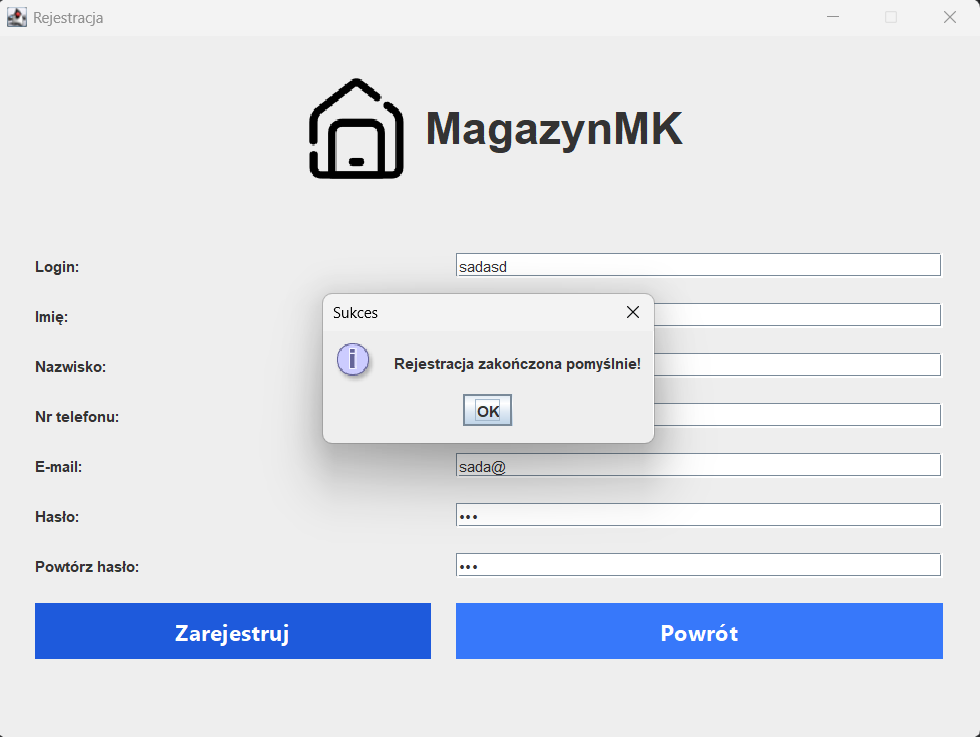
\includegraphics[width=.7\linewidth]{figures/RejestracjaKom5.png}\
    \caption{Komunikat5.\label{Komunikat5}}
\end{figure}
Po kliknięciu ok przechodzi do OknoLogowania
\clearpage
\section{OknoLogowania}
\label{sec:OknoLogowania}
Po kliknięciu w MenuGlowne przycisku Zaloguj lub po zarejestrowaniu się wyskakuje nam okno logowania:
\begin{figure}[H]
    \centering
    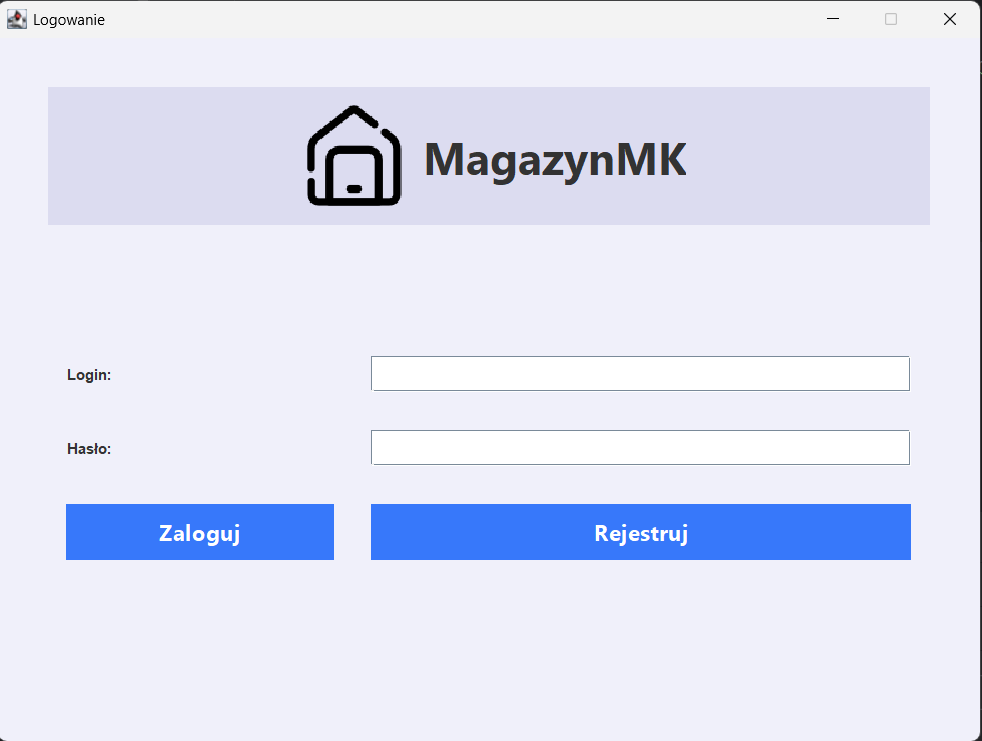
\includegraphics[width=.7\linewidth]{figures/OknoLogowania.png}\
    \caption{OknoLogowania.\label{OknoLogowania}}
\end{figure}
Jeśli wpiszemy niepoprawne dane wyskoczy komunikat:
\begin{figure}[H]
    \centering
    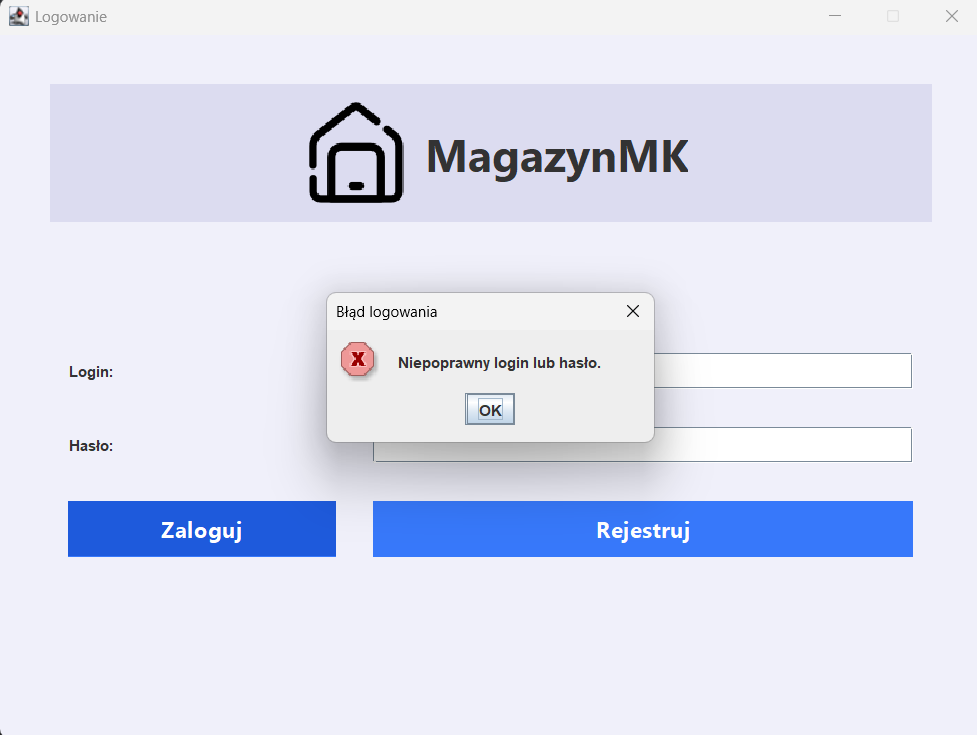
\includegraphics[width=.7\linewidth]{figures/LogowanieKomunikat.png}\
    \caption{Komunikat6.\label{Komunikat6}}
\end{figure}
\clearpage
\section{PanelUzytkownika}
\label{sec:PanelUzytkownika}
Jeśli w oknie logowania zalogujemy się na konto użytkownika nie będącego administratorem wyskoczy nam PanelUzytkownika:
\begin{figure}[H]
    \centering
    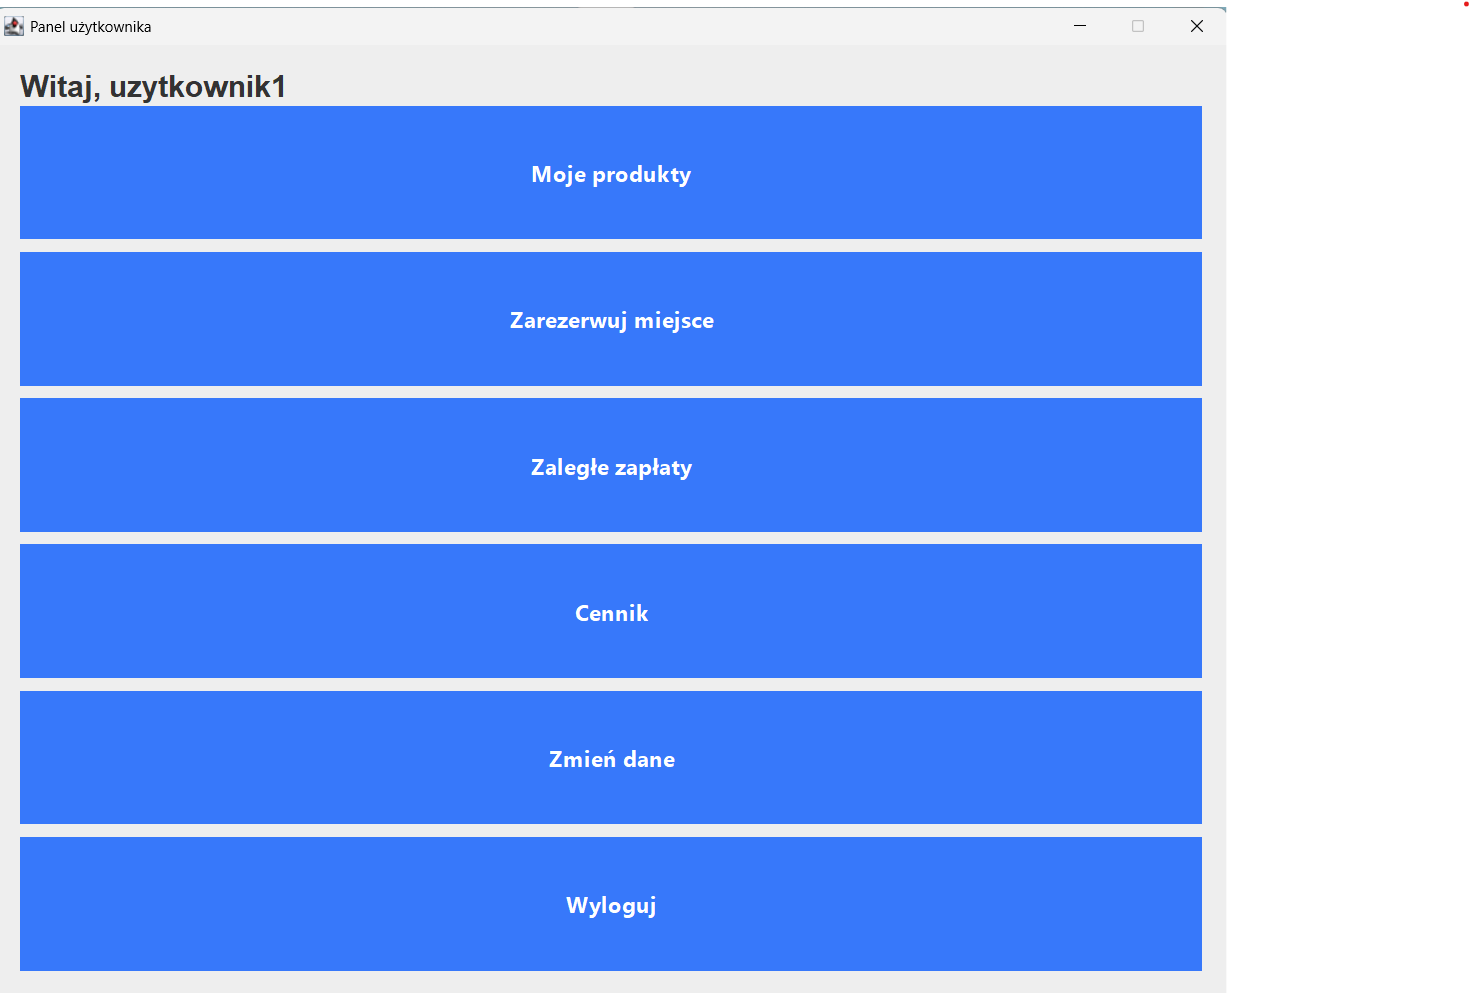
\includegraphics[width=.7\linewidth]{figures/PanelUzytkownika.png}\
    \caption{PanelUzytkownika.\label{PanelUzytkownika}}
\end{figure}
\clearpage
\subsection{Moje produkty}
\label{subsec:Moje produkty}
Po kliknięciu Moje Produkty wyskoczy nam takie okienko:
\begin{figure}[H]
    \centering
    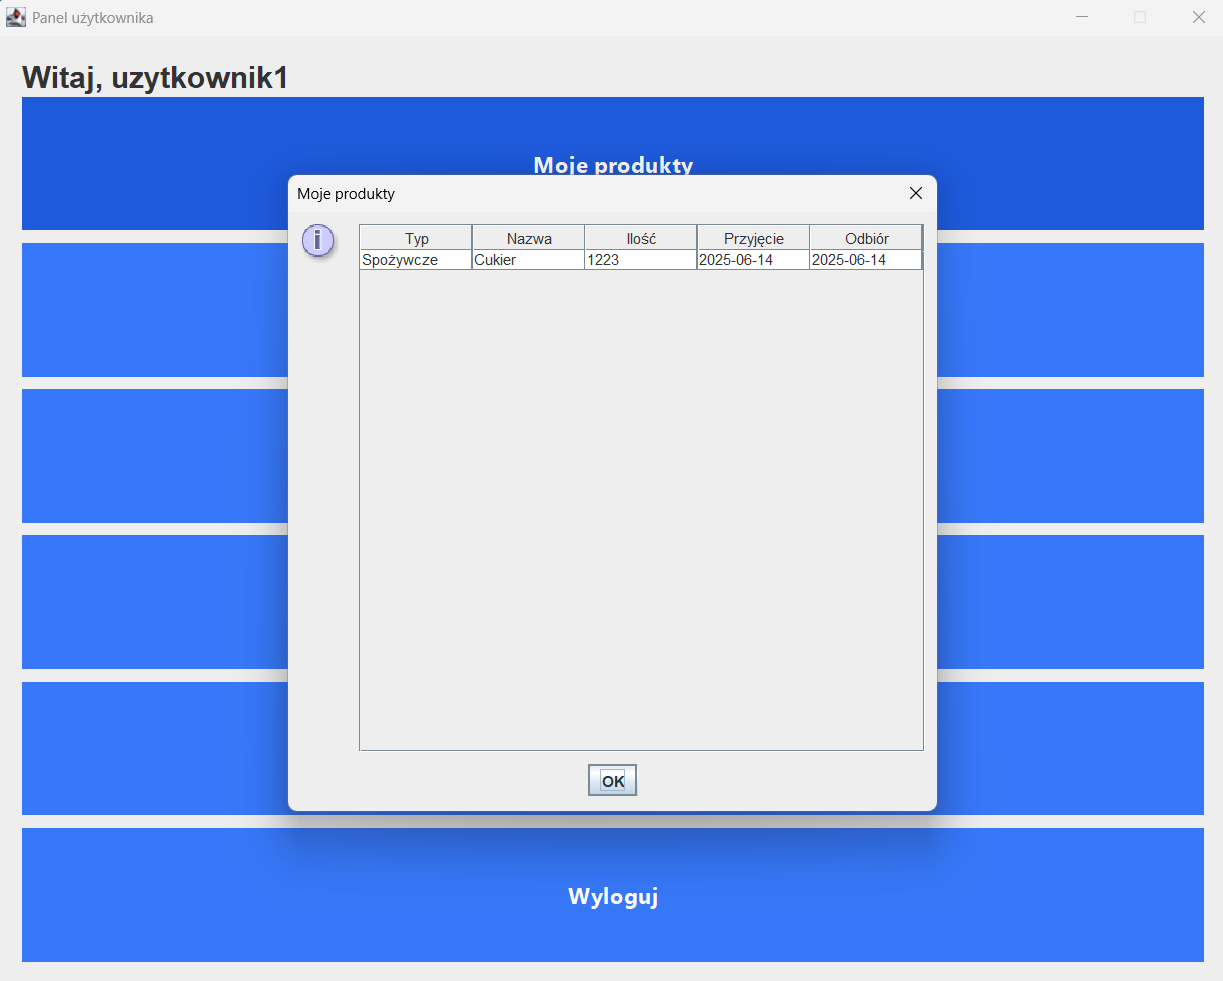
\includegraphics[width=.7\linewidth]{figures/PanelUzytkownika1.png}\
    \caption{PanelUzytkownika1.\label{PanelUzytkownika1}}
\end{figure}
\clearpage
\subsection{Zarezerwuj miejsce}
\label{subsec:Zarezerwuj miejsce}
Po kliknięciu na Zarezerwuj miejsce wyskakuje takie okno:
\begin{figure}[H]
    \centering
    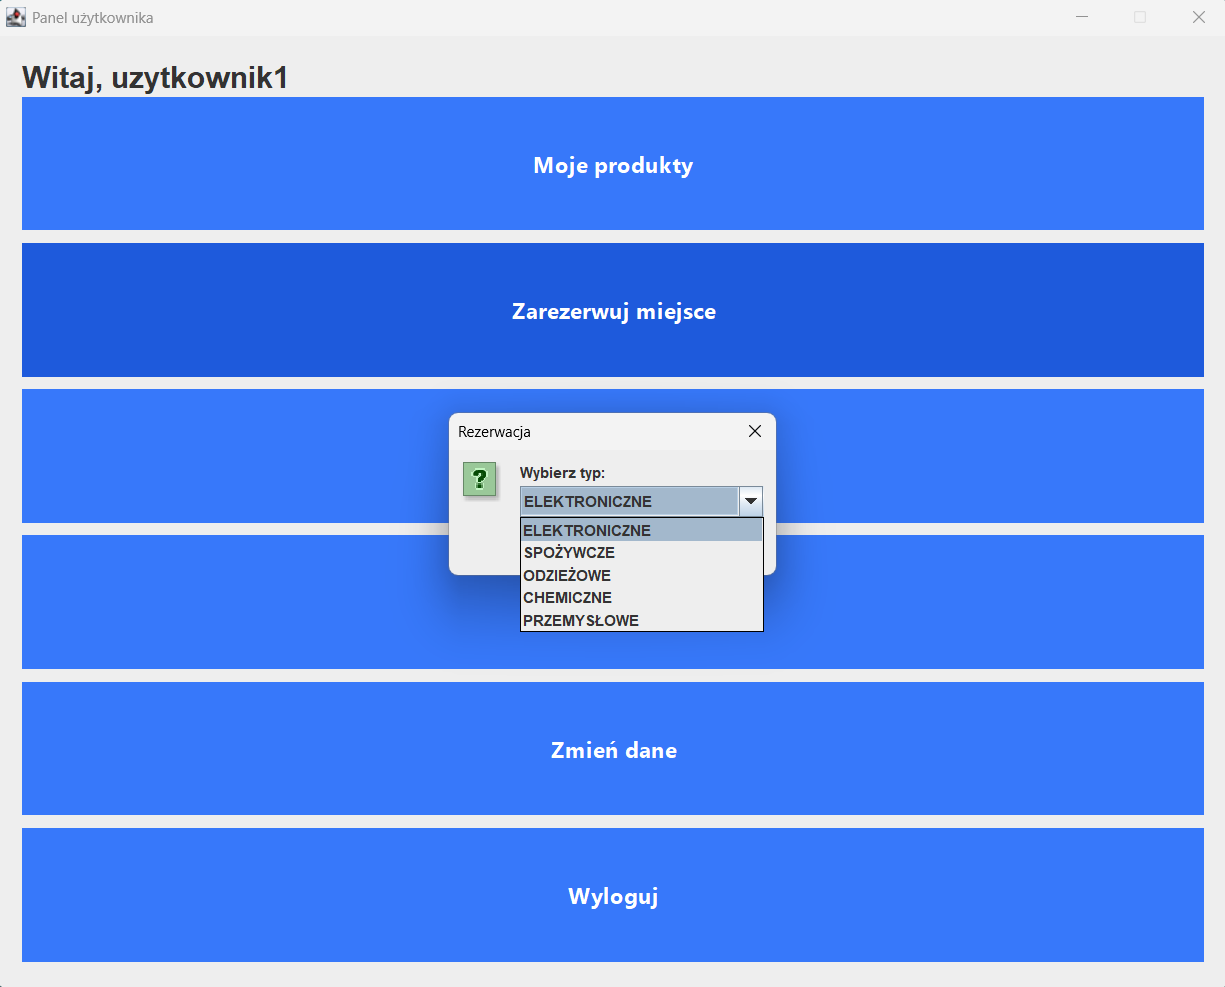
\includegraphics[width=.7\linewidth]{figures/PanelUzytkownika2.png}\
    \caption{PanelUzytkownika2.\label{PanelUzytkownika2}}
\end{figure}
Do każdego typu produktu są przypisane po 3 rodzaje produktów:
ELEKTRONICZNE:
\begin{figure}[H]
    \centering
    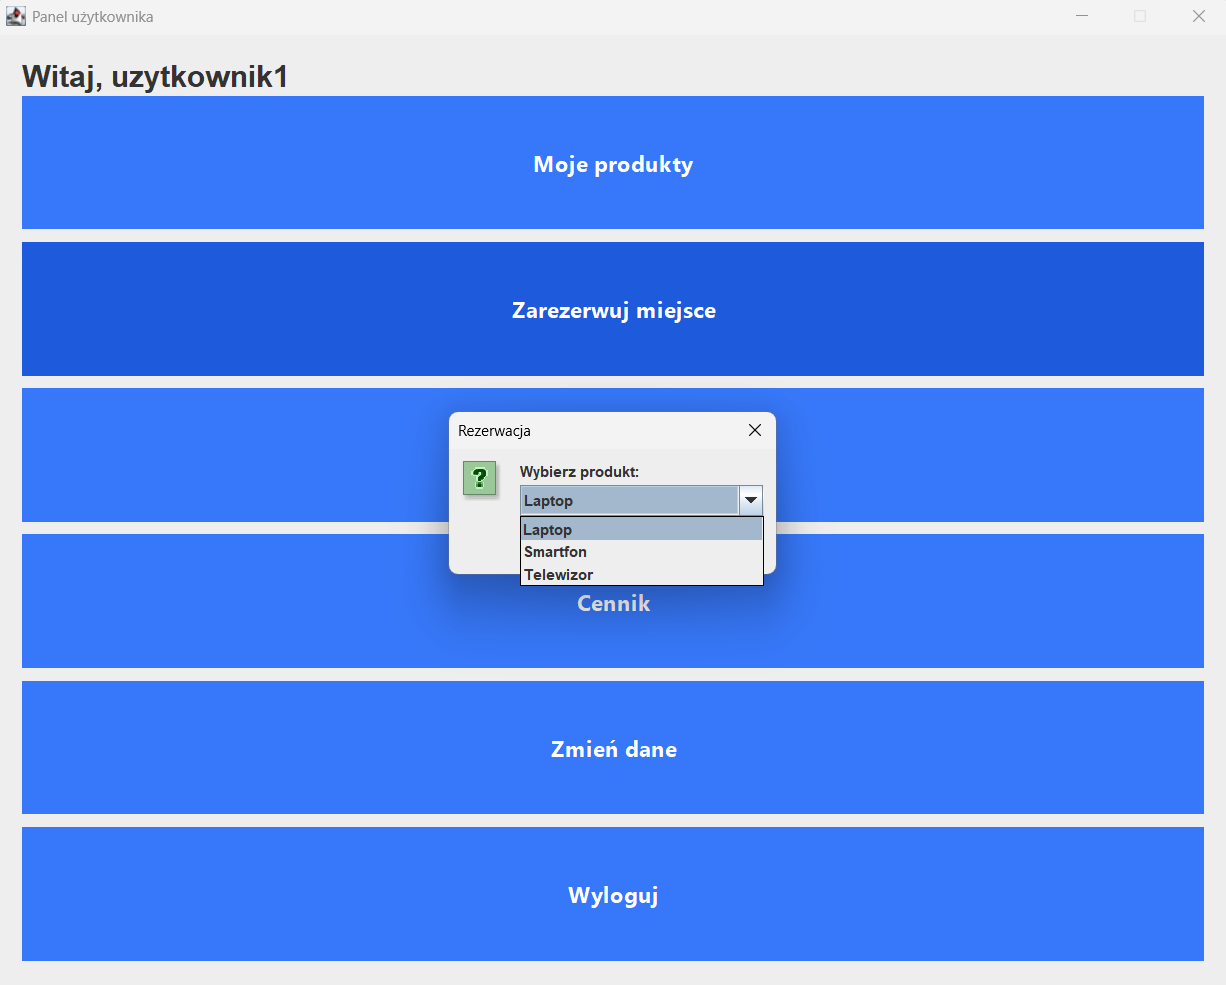
\includegraphics[width=.7\linewidth]{figures/PanelUzytkownika3.png}\
    \caption{PanelUzytkownika3.\label{PanelUzytkownika3}}
\end{figure}
SPOŻYWCZE:
\begin{figure}[H]
    \centering
    \includegraphics[width=.7\linewidth]{figures/PanelUzytkownika9.png}\
    \caption{PanelUzytkownika9.\label{PanelUzytkownika9}}
\end{figure}
ODZIEŻOWE:
\begin{figure}[H]
    \centering
    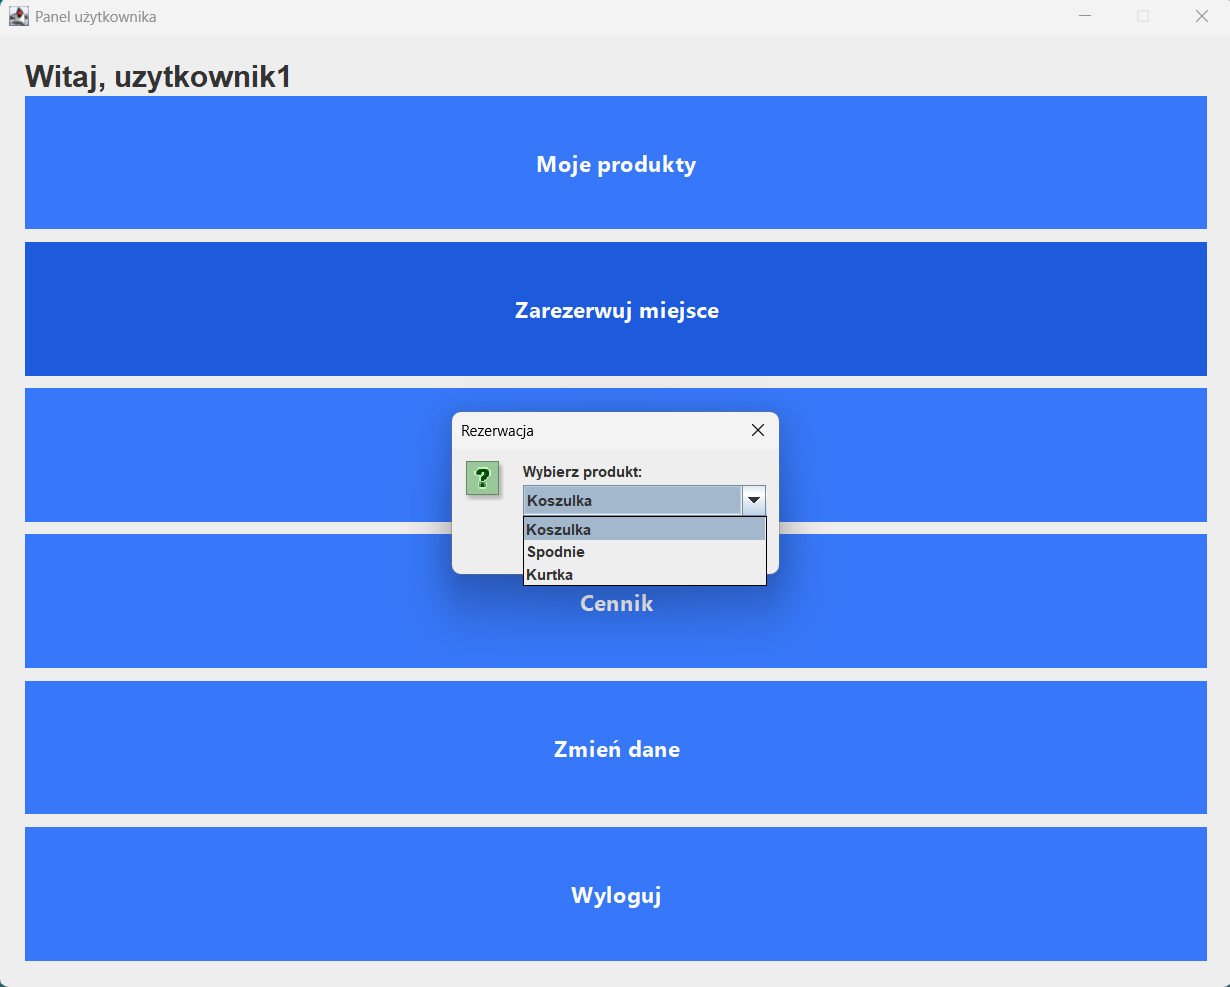
\includegraphics[width=.7\linewidth]{figures/PanelUzytkownika10.png}\
    \caption{PanelUzytkownika10.\label{PanelUzytkownika10}}
\end{figure}
CHEMICZNE:
\begin{figure}[H]
    \centering
    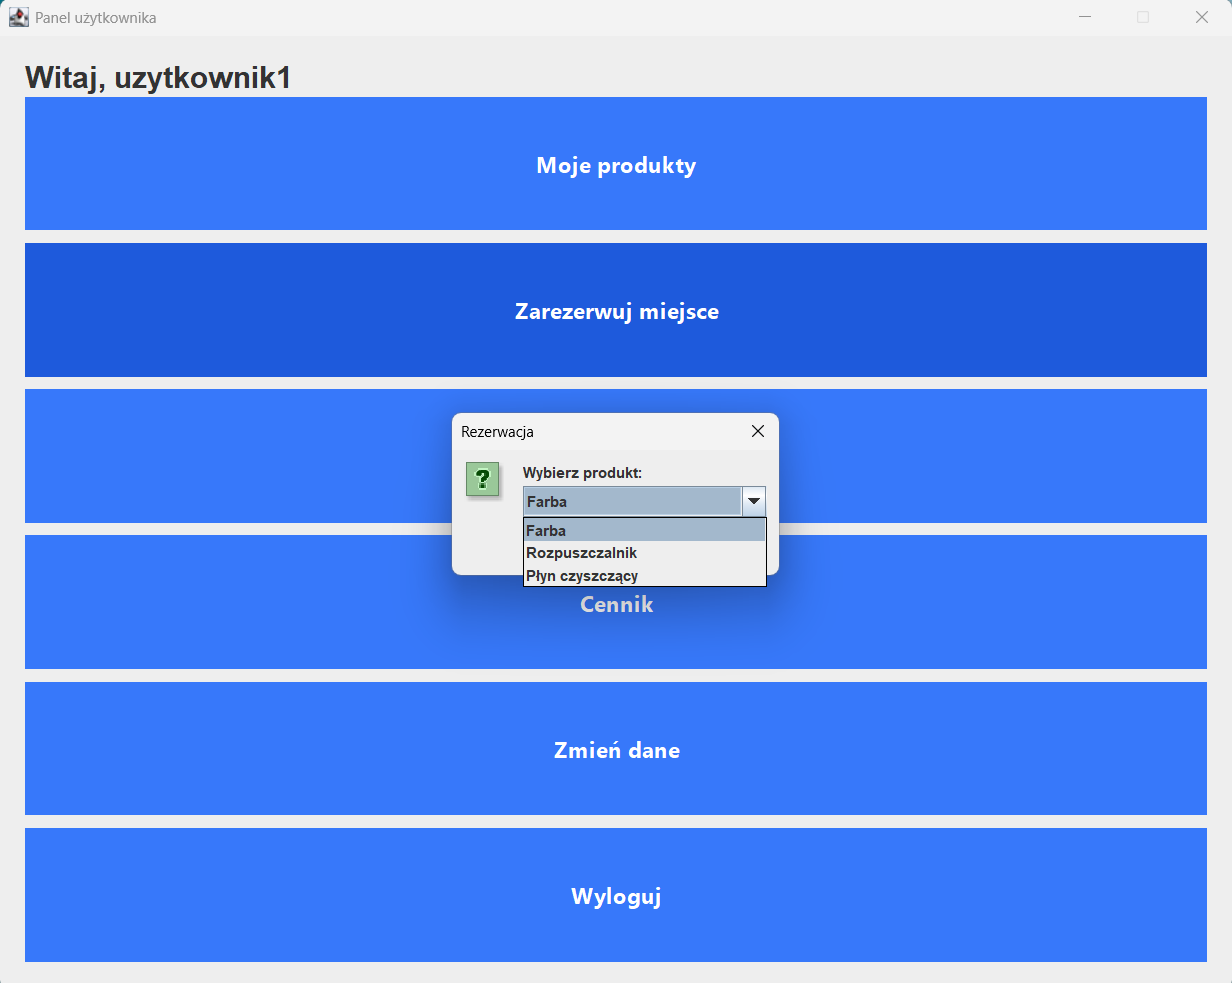
\includegraphics[width=.7\linewidth]{figures/PanelUzytkownika11.png}\
    \caption{PanelUzytkownika11.\label{PanelUzytkownika11}}
\end{figure}
PRZEMYSŁOWE:
\begin{figure}[H]
    \centering
    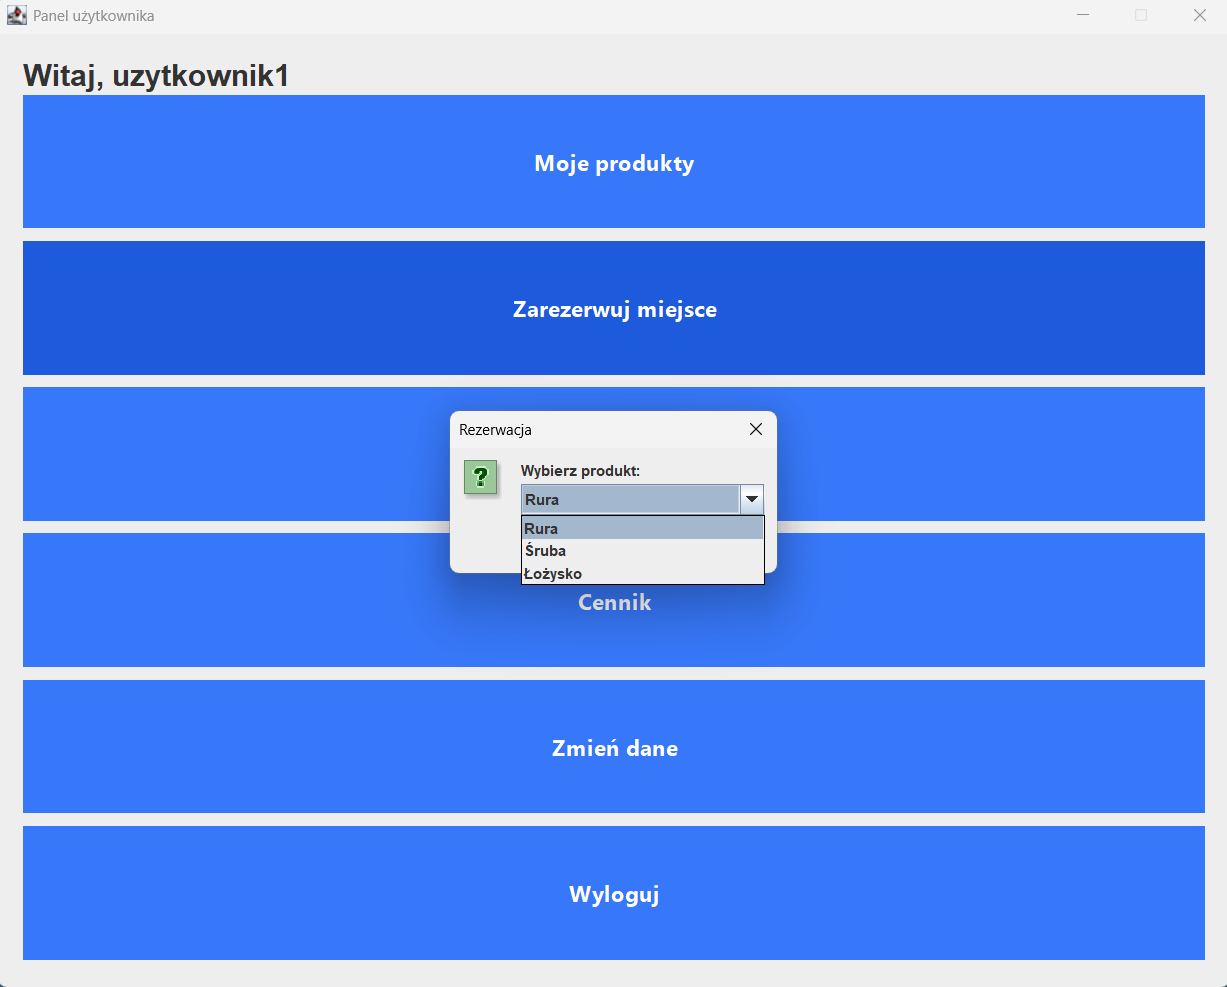
\includegraphics[width=.7\linewidth]{figures/PanelUzytkownika12.png}\
    \caption{PanelUzytkownika12.\label{PanelUzytkownika12}}
\end{figure}
Po wybraniu produktu musimy wpisać ilość:
\begin{figure}[H]
    \centering
    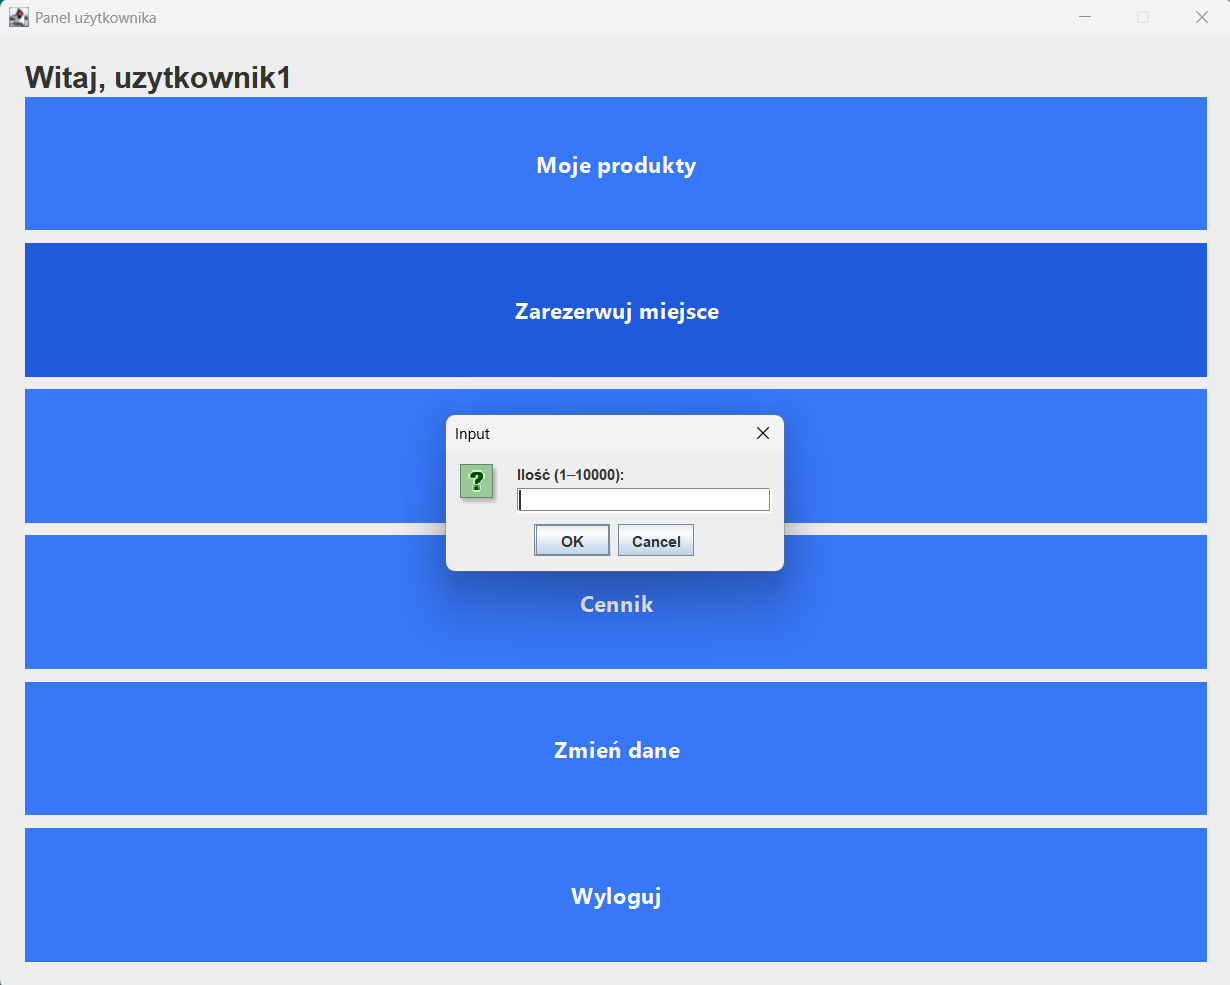
\includegraphics[width=.7\linewidth]{figures/Paneluzytkownika4.png}\
    \caption{PanelUzytkownika4.\label{PanelUzytkownika4}}
\end{figure}
Jeśli ilość przekroczy 10000, to wyskoczy taki komunikat:
\begin{figure}[H]
    \centering
    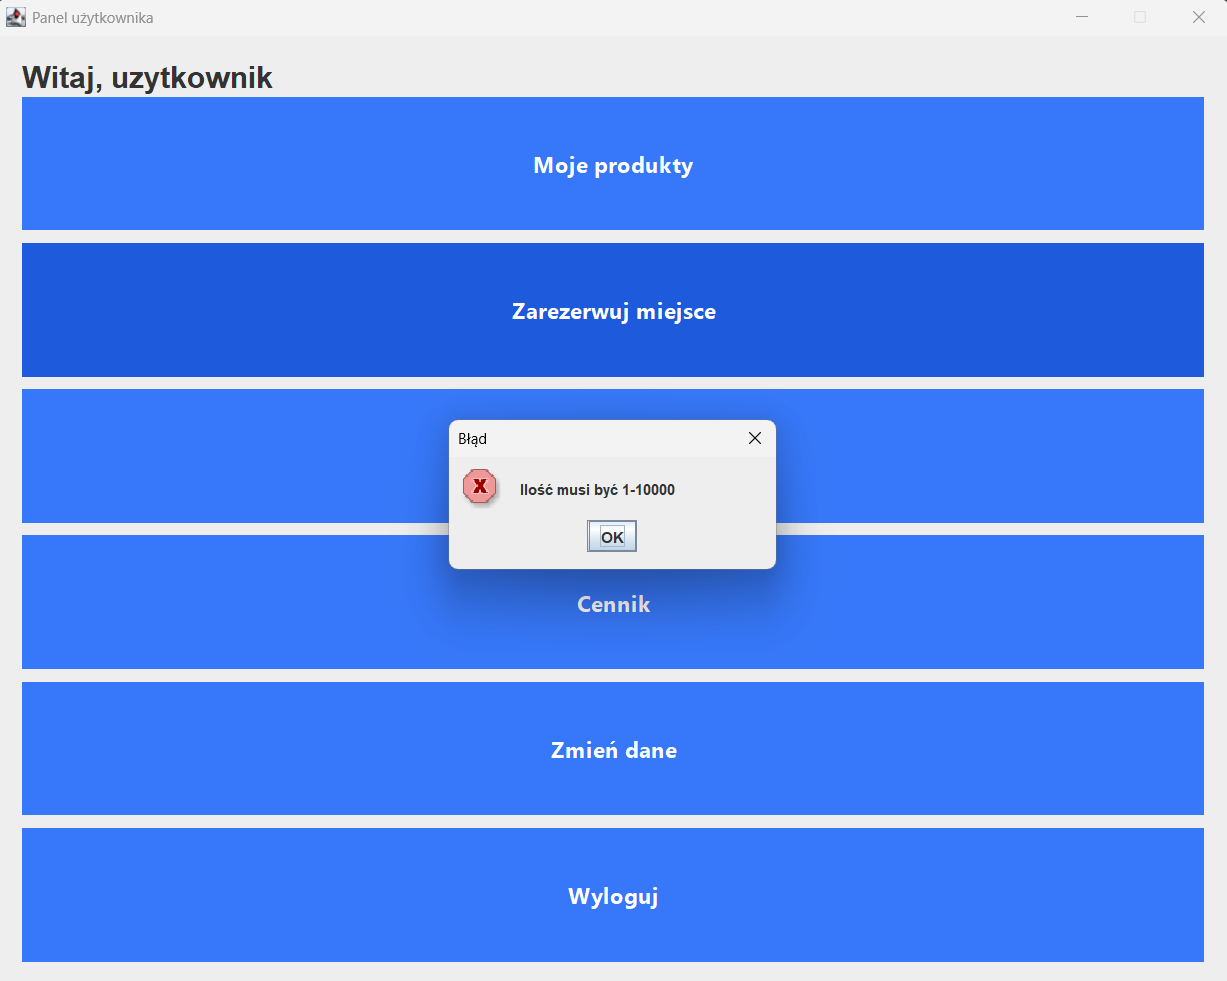
\includegraphics[width=.7\linewidth]{figures/PanelUzytkownika23.png}\
    \caption{PanelUzytkownika23.\label{PanelUzytkownika23}}
\end{figure}
Następnie należy wybrać daty od kiedy do kiedy rezerwujemy miejsce:
\begin{figure}[H]
    \centering
    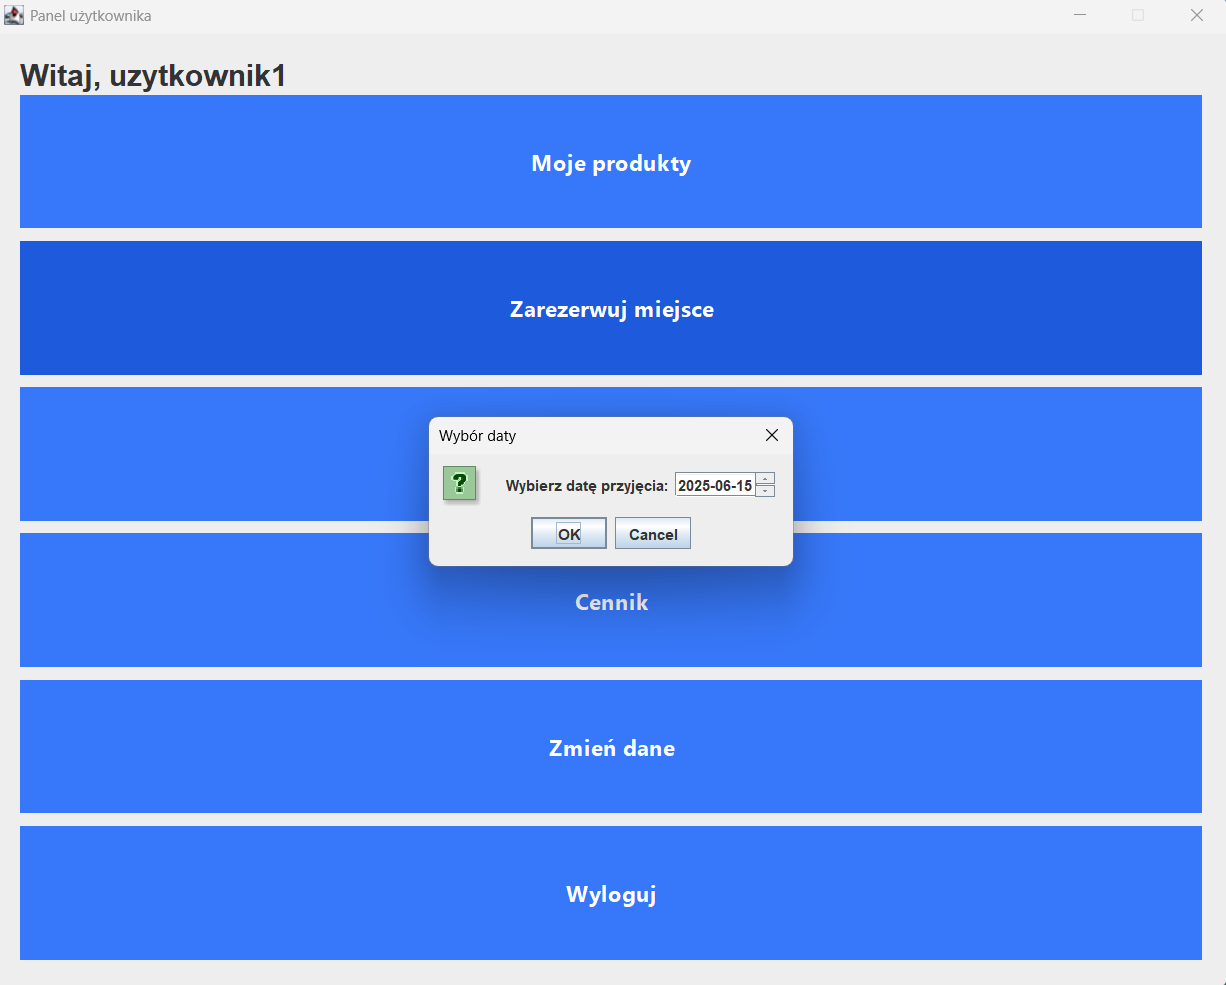
\includegraphics[width=.7\linewidth]{figures/PanelUzytkownika5.png}\
    \caption{PanelUzytkownika5.\label{PanelUzytkownika5}}
\end{figure}
\begin{figure}[H]
    \centering
    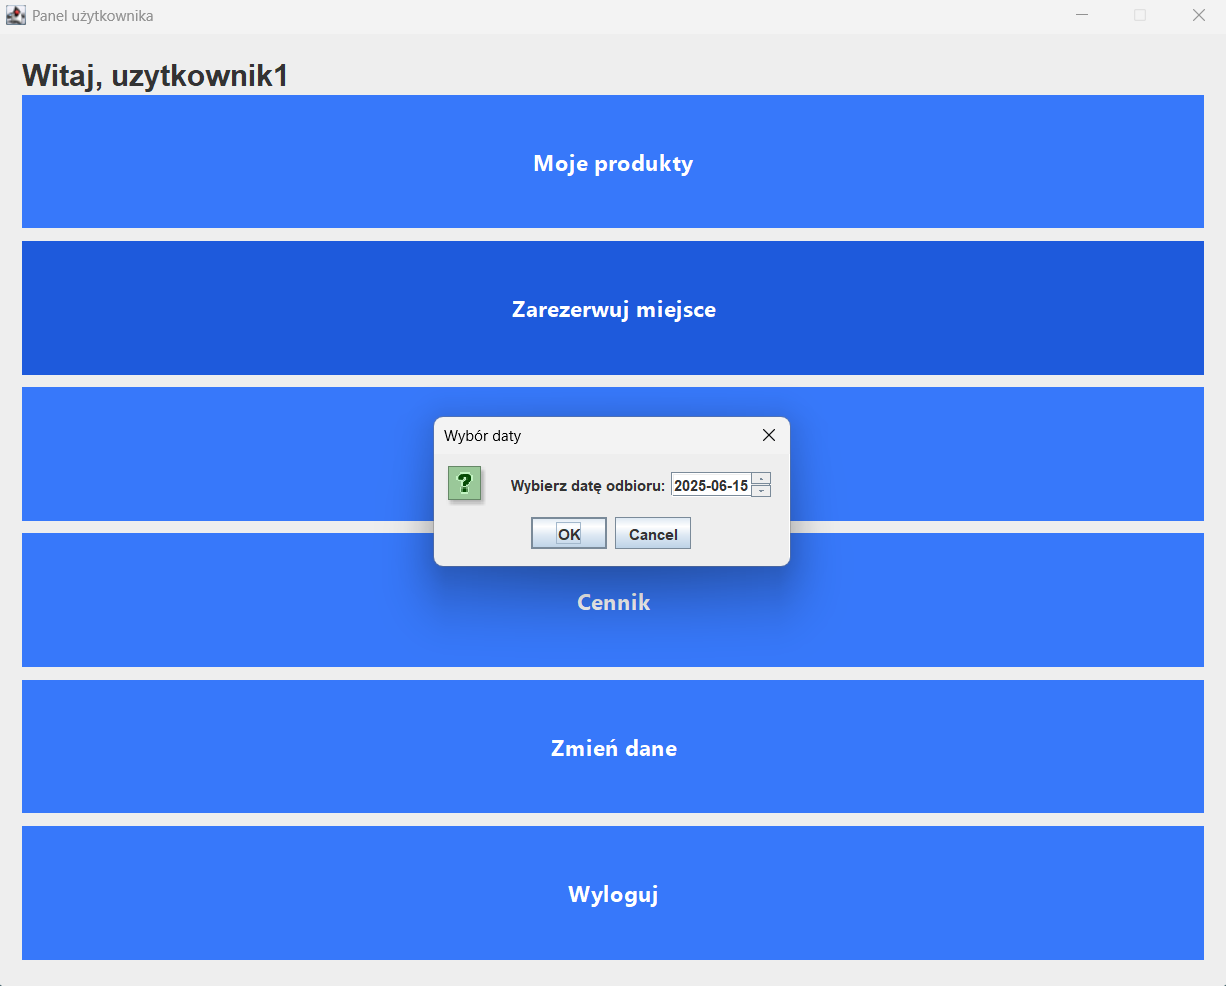
\includegraphics[width=.7\linewidth]{figures/PanelUzytkownika6.png}\
    \caption{PanelUzytkownika6.\label{PanelUzytkownika6}}
\end{figure}
Następnie wyświetla 2 komunikaty:
\begin{figure}[H]
    \centering
    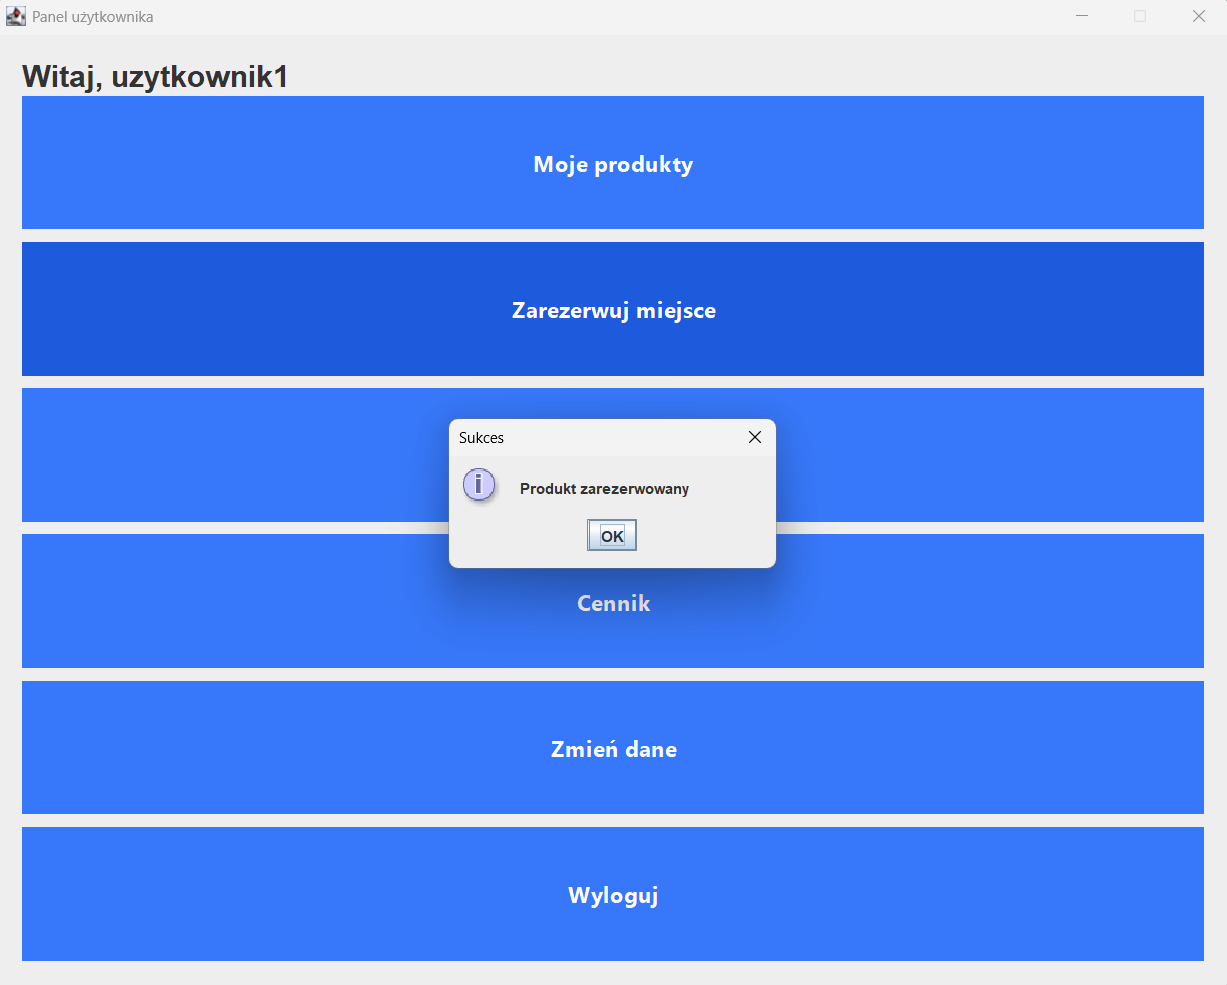
\includegraphics[width=.7\linewidth]{figures/PanelUzytkownika7.png}\
    \caption{PanelUzytkownika7.\label{PanelUzytkownika7}}
\end{figure}
Drugi komunikat mówi nam o kwocie(oblicza ją według cennika) oraz informuje o adresie na którym trzeba uiścić opłatę:
\begin{figure}[H]
    \centering
    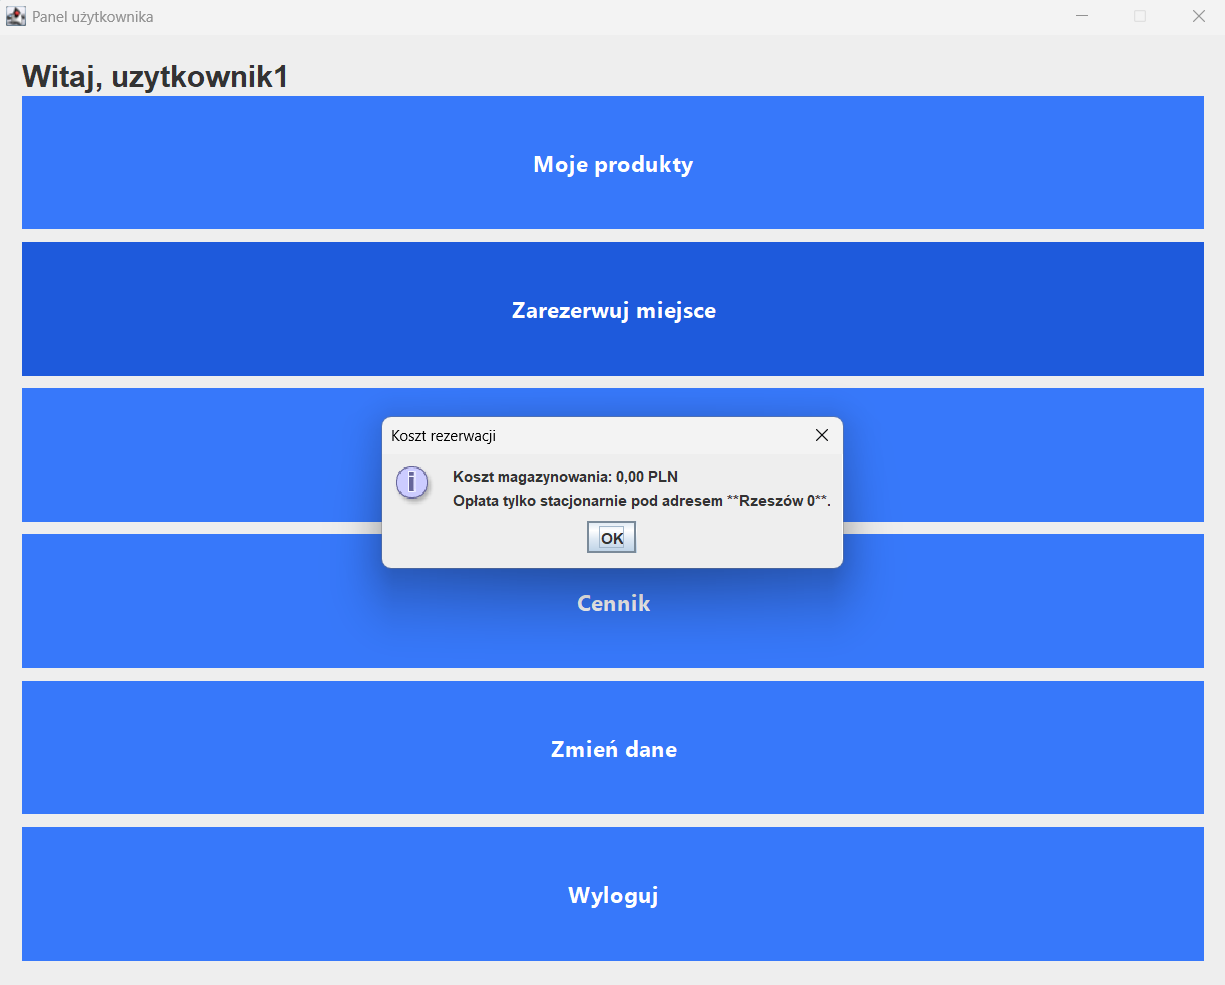
\includegraphics[width=.7\linewidth]{figures/PanelUzytkownika8.png}\
    \caption{PanelUzytkownika8.\label{PanelUzytkownika8}}
\end{figure}
\clearpage
\subsection{Zaległe kary}
\label{subsec:Zaległe kary}
Po kliknięciu na Zaległe zapłaty wyświetli nam się tabela:
\begin{figure}[H]
    \centering
    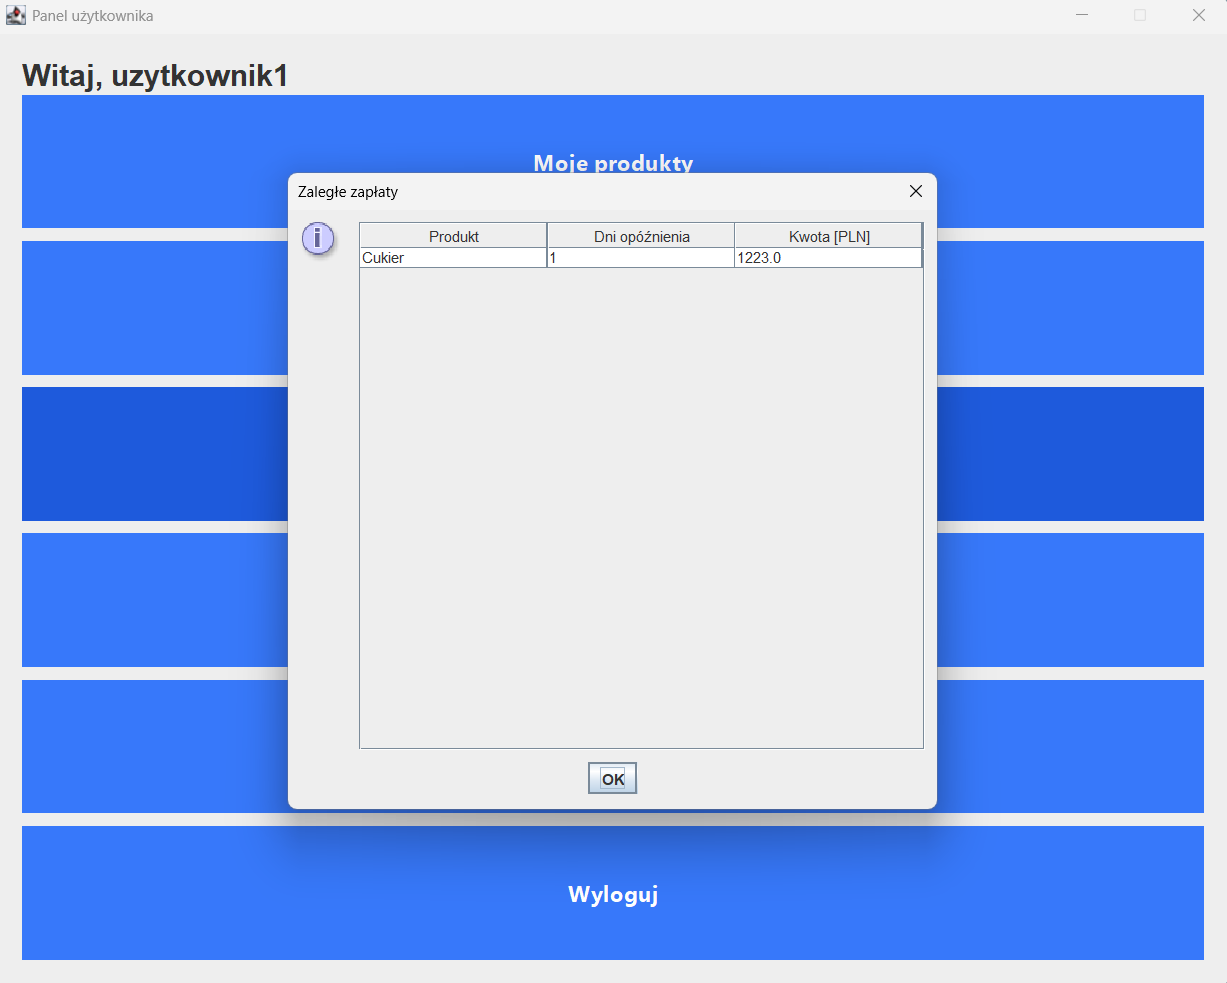
\includegraphics[width=.7\linewidth]{figures/PanelUzytkownika13.png}\
    \caption{PanelUzytkownika13.\label{PanelUzytkownika13}}
\end{figure}
\clearpage
\subsection{Cennik}
\label{subsec:Cennik}
Jeśli klikniemy na cennik to wyświetli nam się tabela:
\begin{figure}[H]
    \centering
    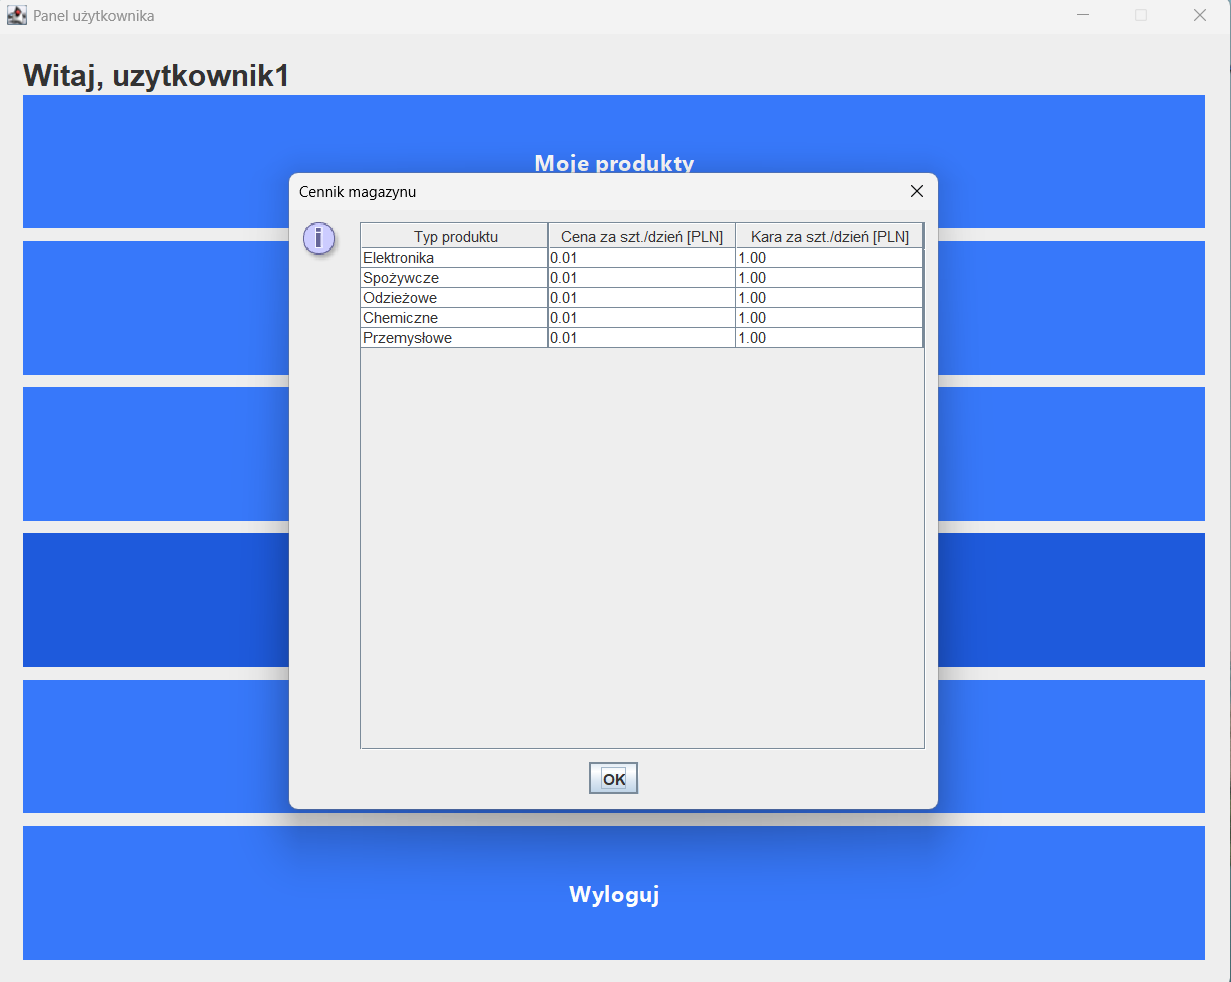
\includegraphics[width=.7\linewidth]{figures/PanelUzytkownika14.png}\
    \caption{PanelUzytkownika14.\label{PanelUzytkownika14}}
\end{figure}
\clearpage
\subsection{Zmień dane}
\label{subsec:Zmień dane}
Jeśli klikniemy na zmień dane to wyświetli się takie okno:
\begin{figure}[H]
    \centering
    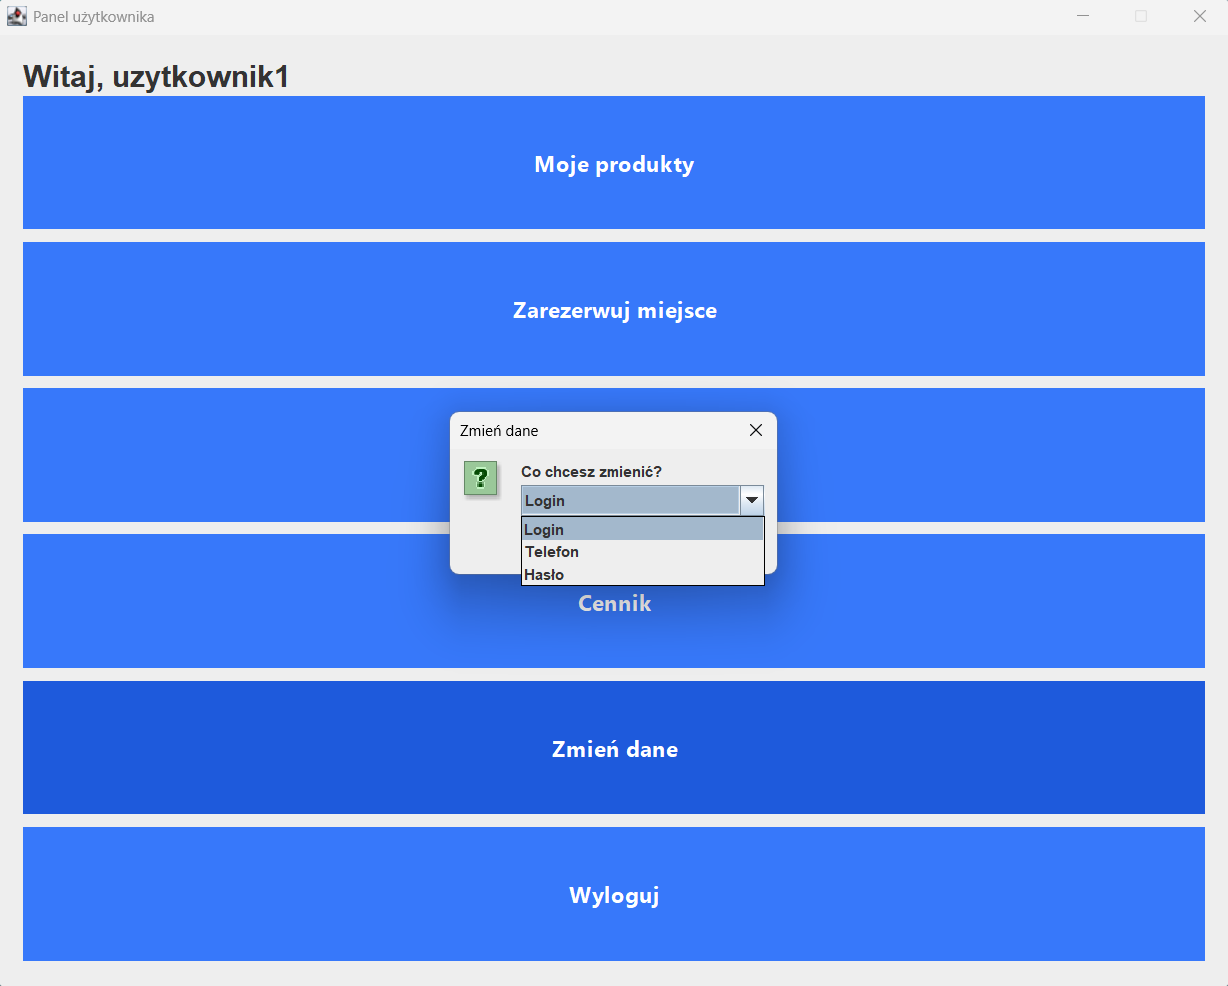
\includegraphics[width=.7\linewidth]{figures/PanelUzytkownika15.png}\
    \caption{PanelUzytkownika15.\label{PanelUzytkownika15}}
\end{figure}
Jeśli przy zmienianiu loginu nie będzie on miał 4 liter to wyświetli taki komunikat:
\begin{figure}[H]
    \centering
    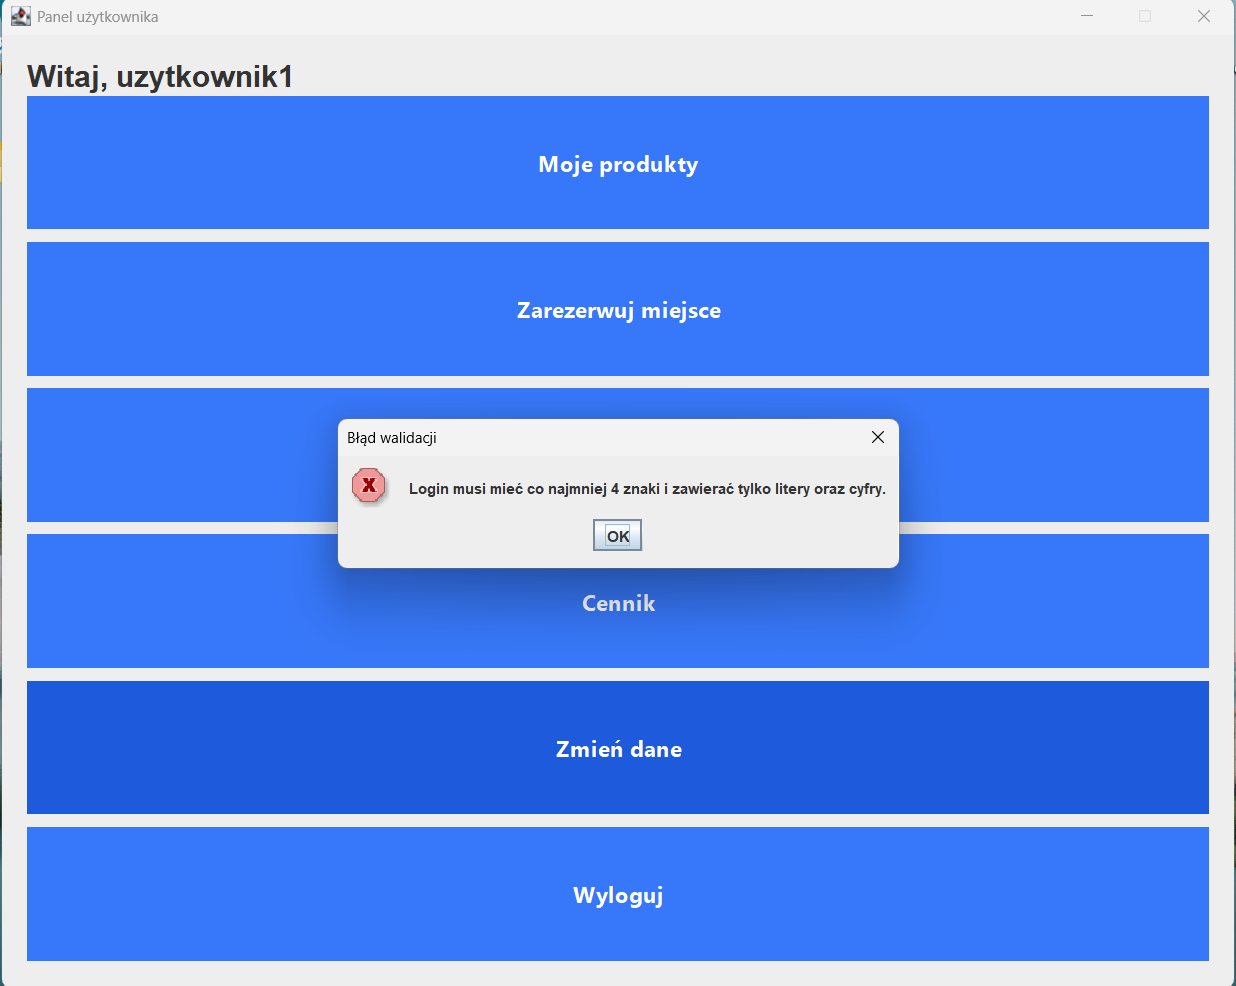
\includegraphics[width=.7\linewidth]{figures/PanelUzytkownika16.png}\
    \caption{PanelUzytkownika16.\label{PanelUzytkownika16}}
\end{figure}
Jeśli jednak login zostanie wpisany poprawnie to wyświetli się taki komunikat:
\begin{figure}[H]
    \centering
    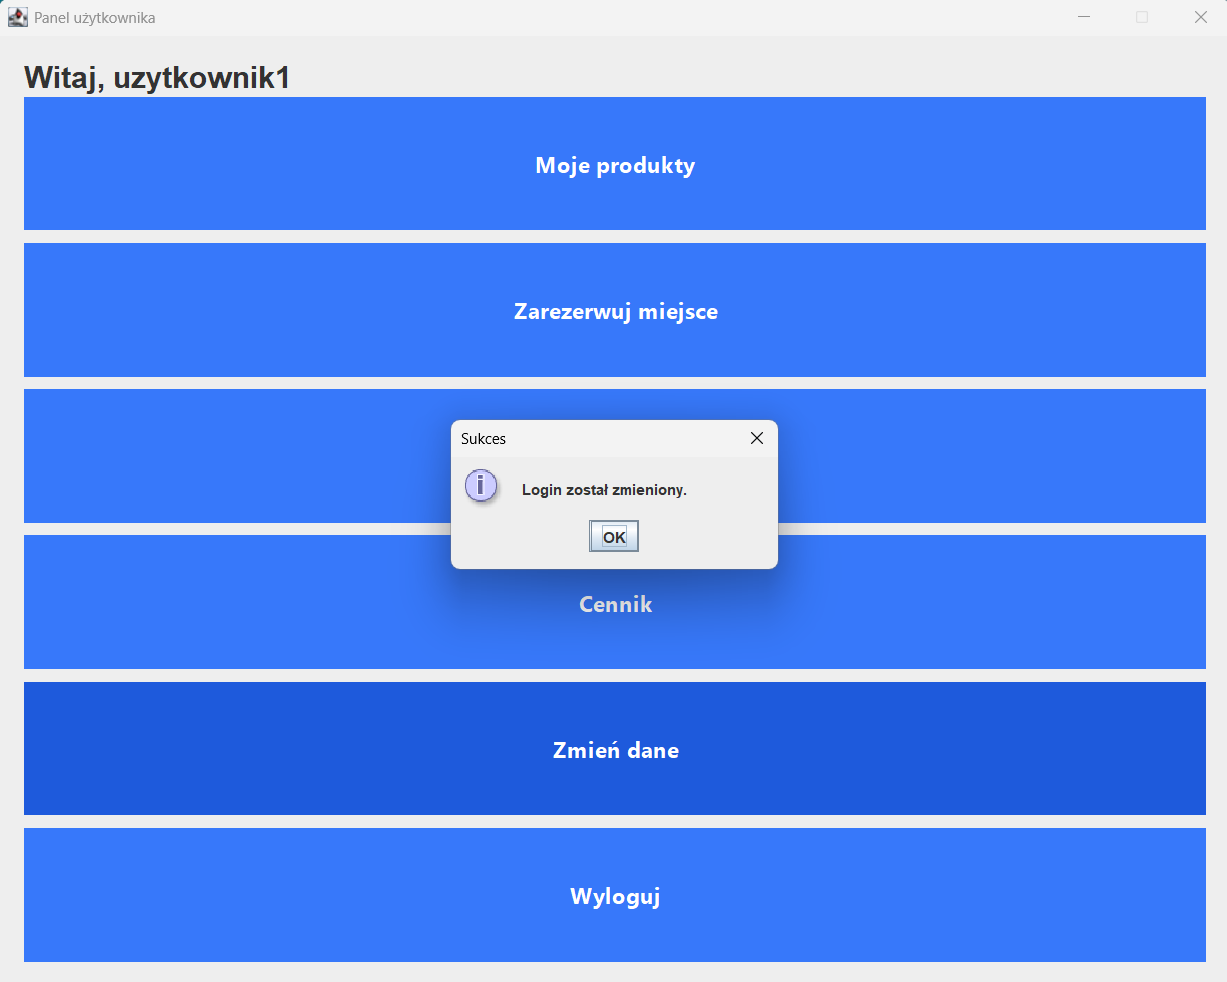
\includegraphics[width=.7\linewidth]{figures/PanelUzytkownika17.png}\
    \caption{PanelUzytkownika17.\label{PanelUzytkownika17}}
\end{figure}
Jeśli przy zmianie Nr.Tel nie będzie od 9 do 11 liter wyświetli taki komunikat:
\begin{figure}[H]
    \centering
    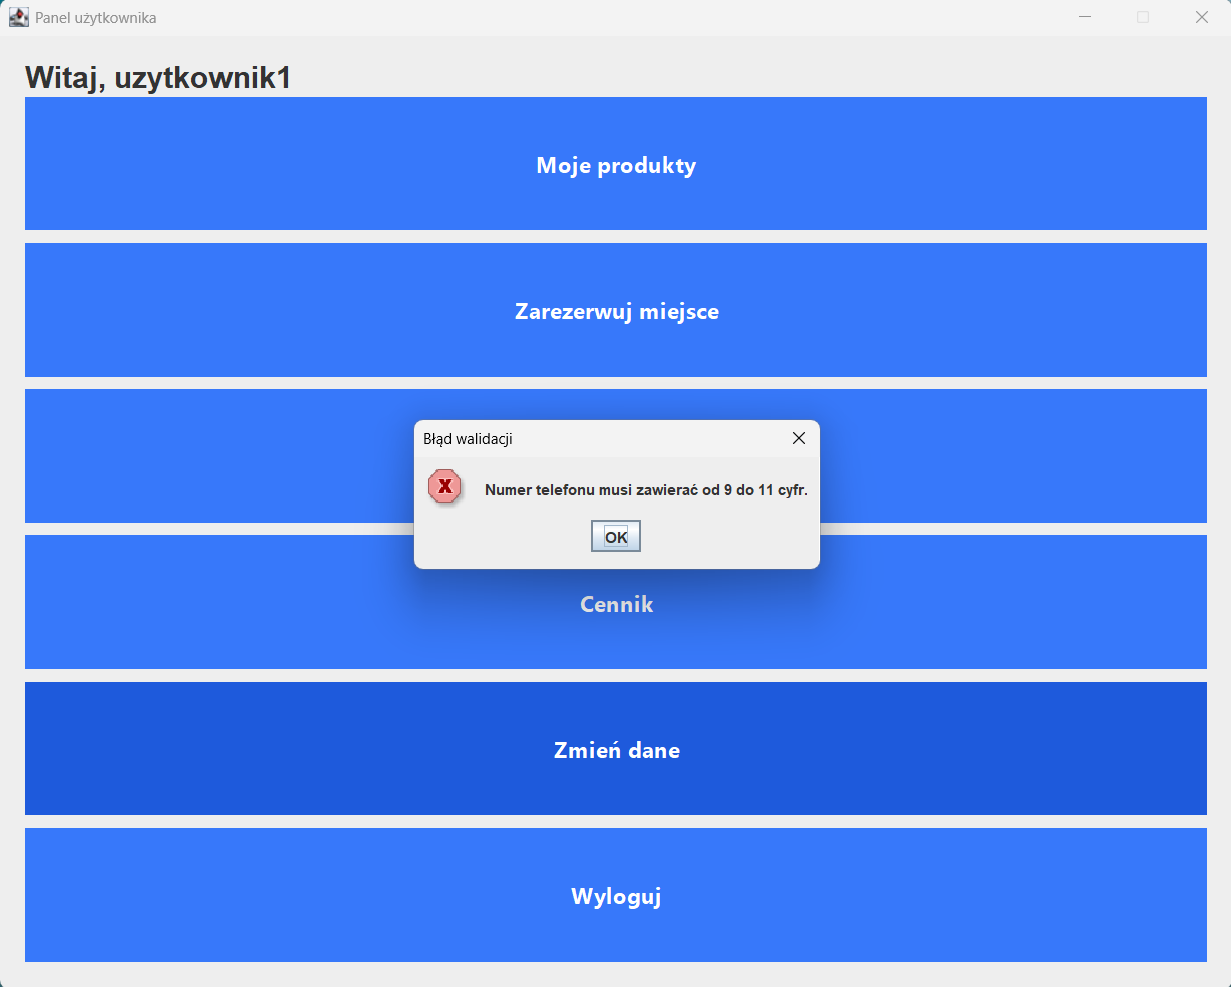
\includegraphics[width=.7\linewidth]{figures/PanelUzytkownika18.png}\
    \caption{PanelUzytkownika18.\label{PanelUzytkownika18}}
\end{figure}
Natomiast gdy użytkownik dobrze wpisze nowy Nr.Tel. wyświetli taki komunikat:
\begin{figure}[H]
    \centering
    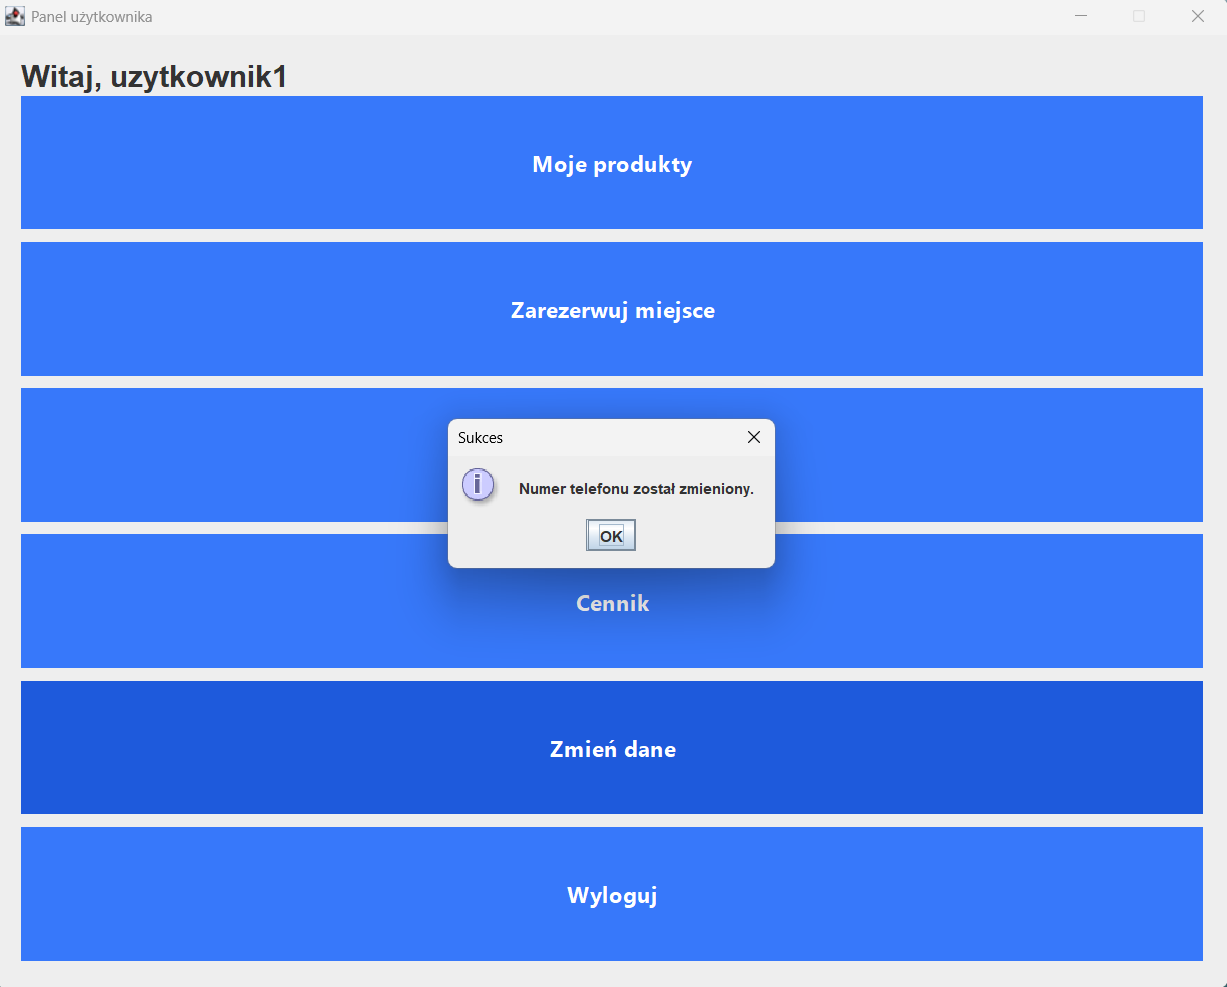
\includegraphics[width=.7\linewidth]{figures/PanelUzytkownika19.png}\
    \caption{PanelUzytkownika19.\label{PanelUzytkownika19}}
\end{figure}
Po wybraniu zmiany hasła, gdy nie będą się one pokrywać, wyświetli taki komunikat:
\begin{figure}[H]
    \centering
    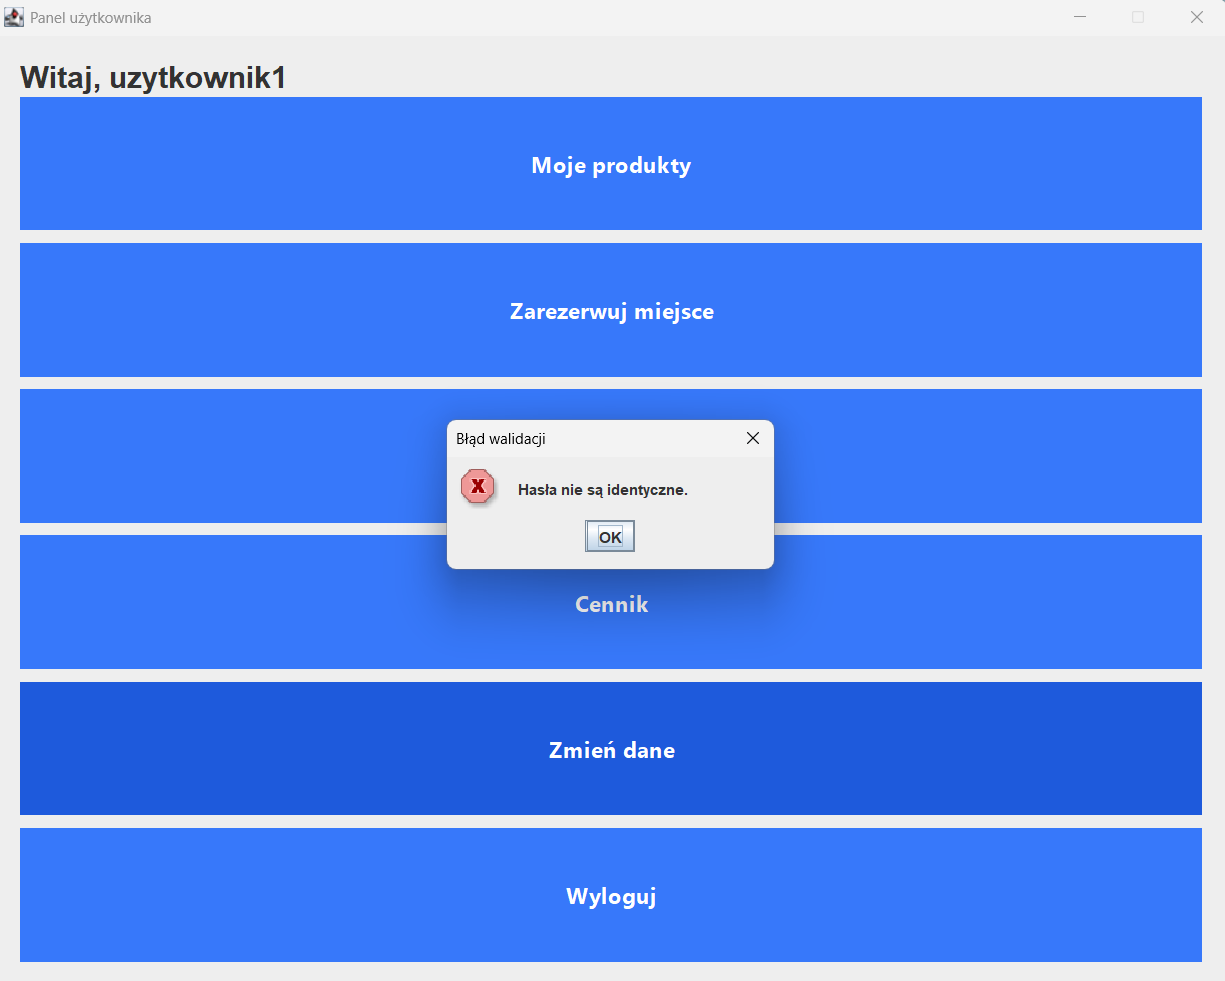
\includegraphics[width=.7\linewidth]{figures/PanelUzytkownika20.png}\
    \caption{PanelUzytkownika20.\label{PanelUzytkownika20}}
\end{figure}
Jeśli hasła się pokrywają:
\begin{figure}[H]
    \centering
    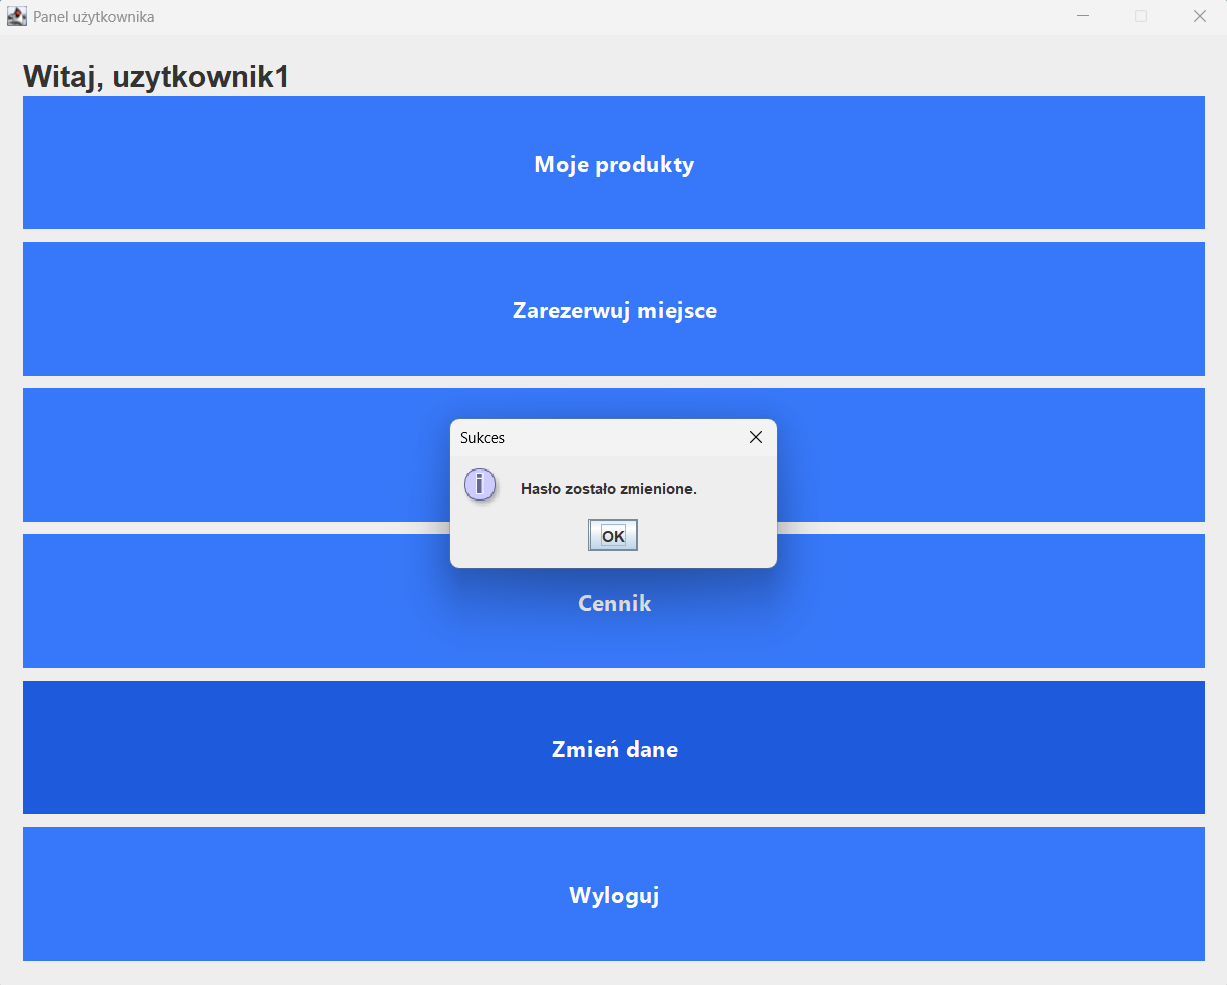
\includegraphics[width=.7\linewidth]{figures/PanelUzytkownika21.png}\
    \caption{PanelUzytkownika21.\label{PanelUzytkownika21}}
\end{figure}
\clearpage
\subsection{Wyloguj}
\label{subsec:Wyloguj}
Po kliknięciu przycisku Wyloguj wyświetli się komunikat:
\begin{figure}[H]
    \centering
    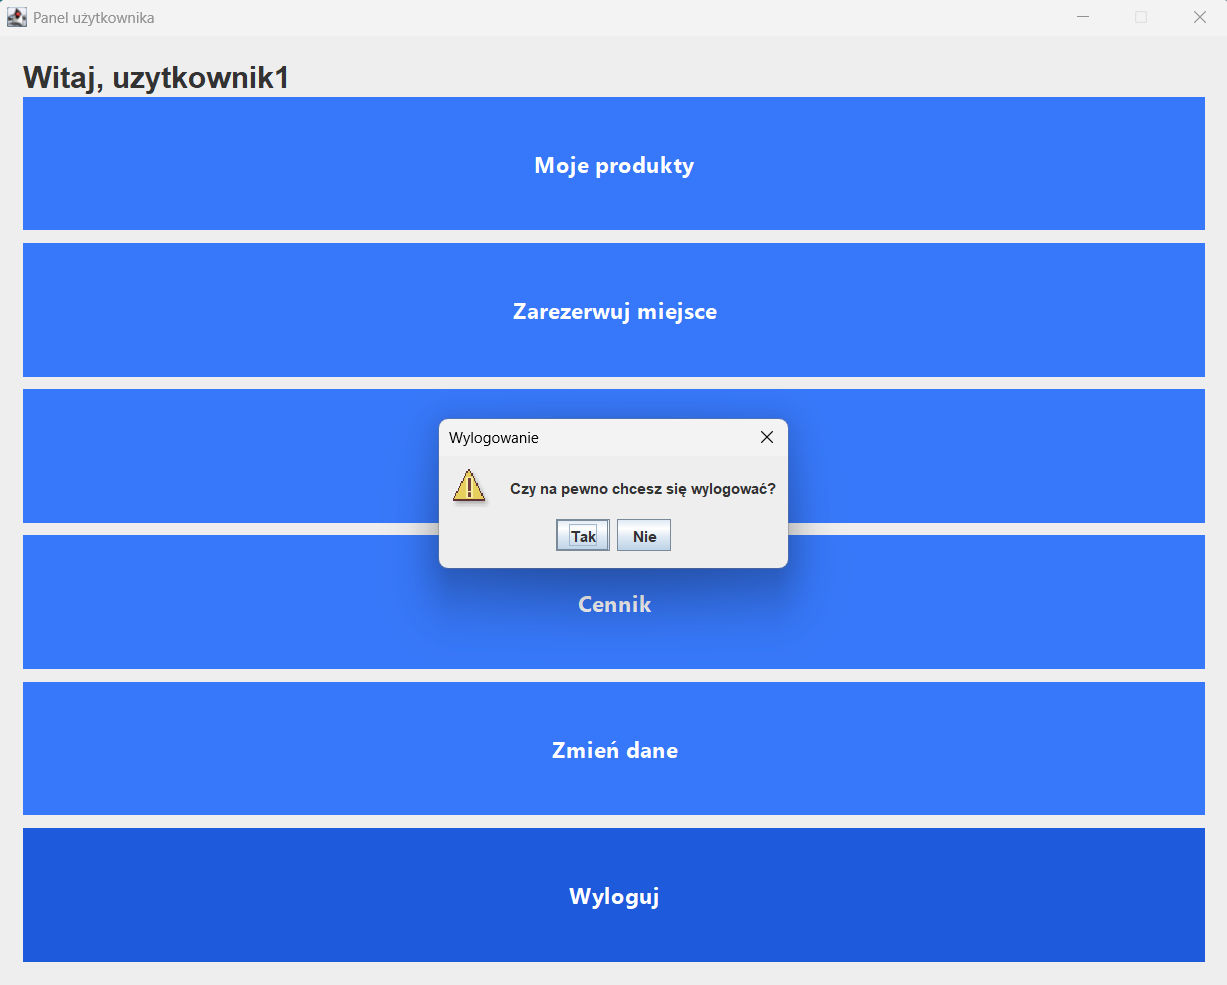
\includegraphics[width=.7\linewidth]{figures/PanelUzytkownika22.png}\
    \caption{PanelUzytkownika22.\label{PanelUzytkownika22}}
\end{figure}
\clearpage
\section{PanelAdministratora}
\label{sec:PanelAdministratora}
Jeśli w oknie logowania zalogujemy się na konto użytkownika będącego administratorem wyskoczy nam PanelAdministratora:
\begin{figure}[H]
    \centering
    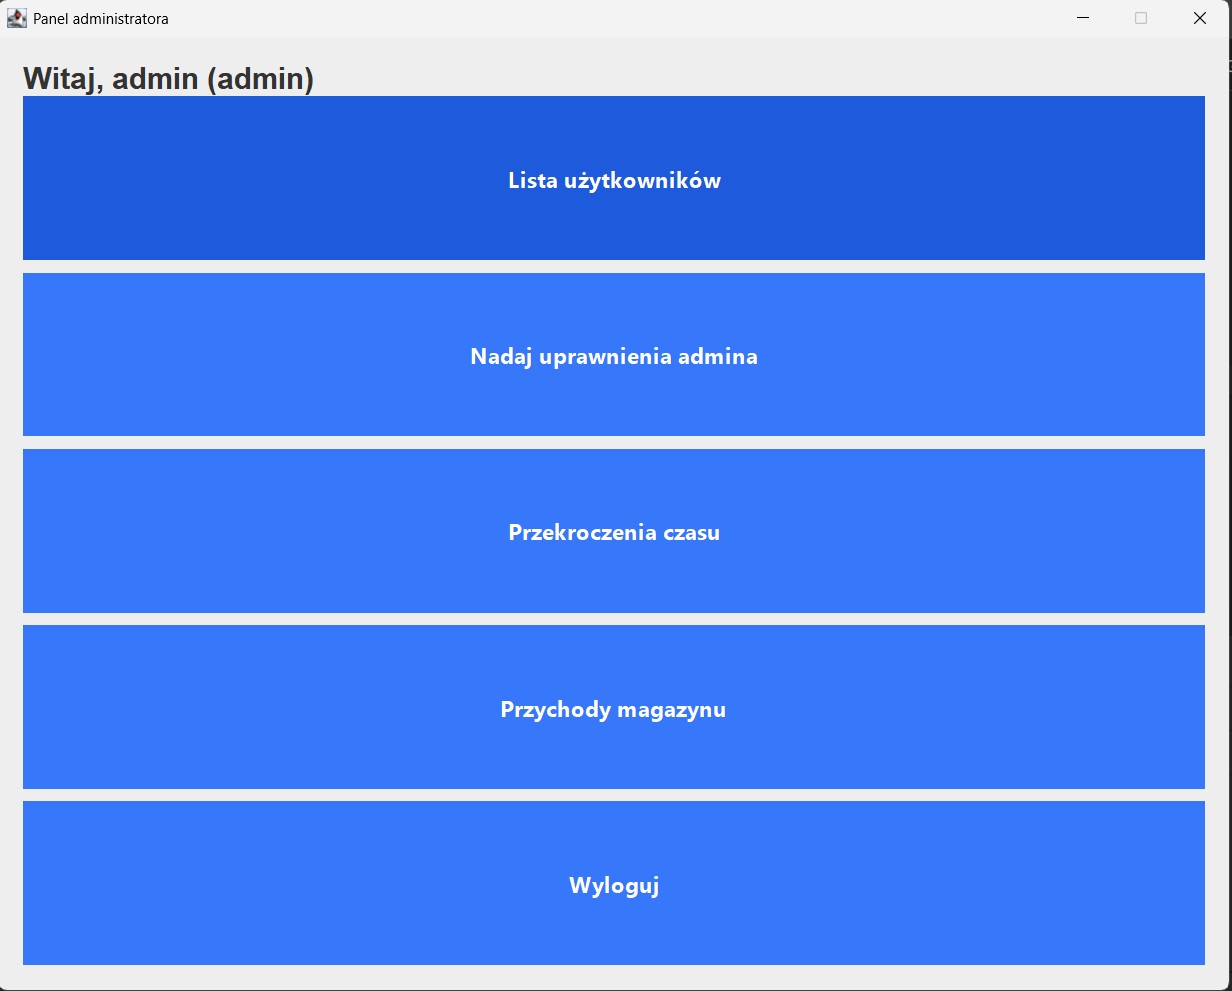
\includegraphics[width=.7\linewidth]{figures/PanelAdministratora.png}\
    \caption{PanelAdministratora.\label{PanelAdministratora}}
\end{figure}
\clearpage
\subsection{Lista użytkowników}
\label{subsec:Lista użytkowników}
Po kliknięciu na Lista użytkowników wyświetli się lista użytkowników wraz z ich produktami
\begin{figure}[H]
    \centering
    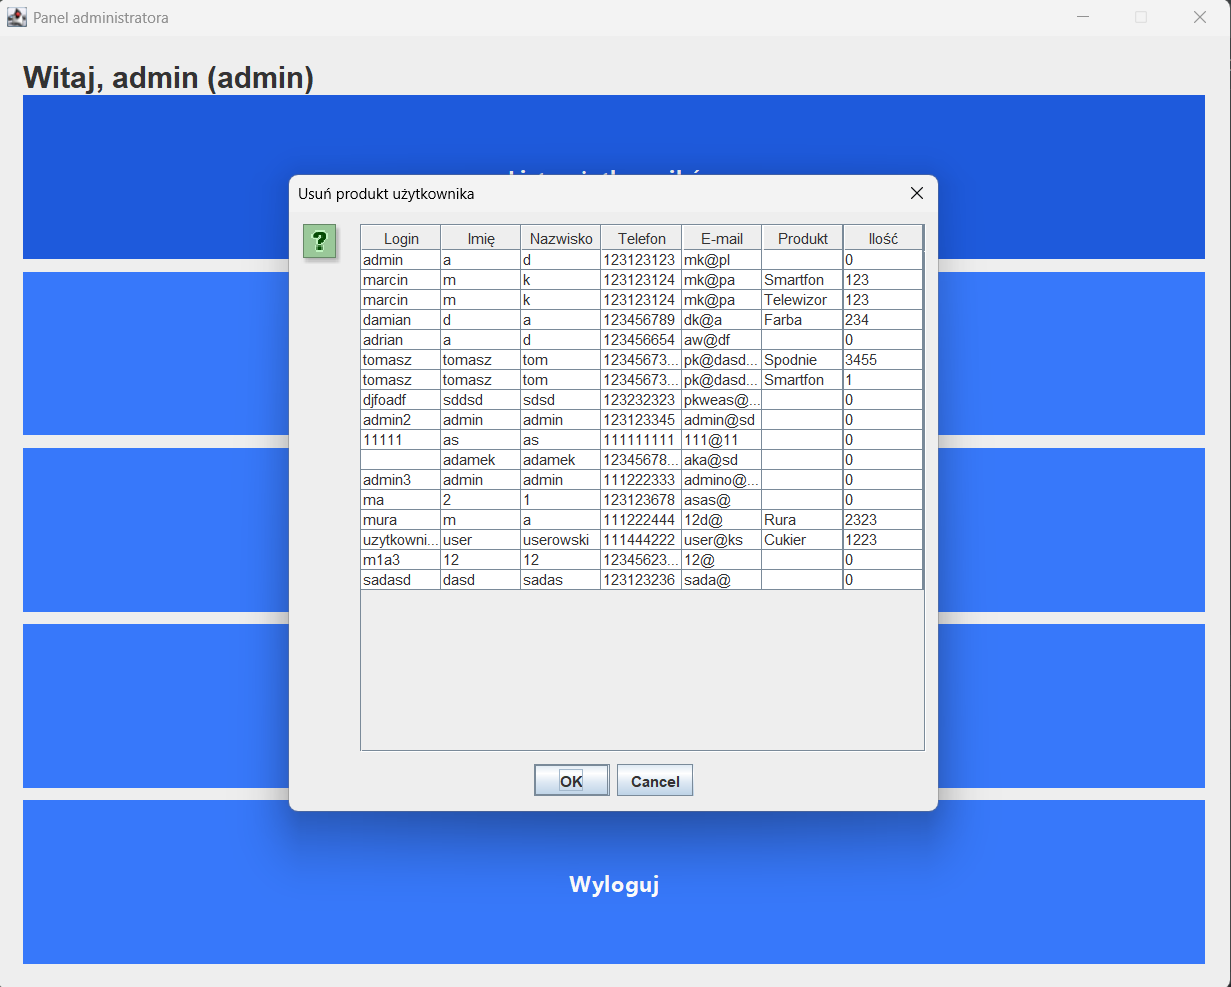
\includegraphics[width=.7\linewidth]{figures/PanelAdministratora1.png}\
    \caption{PanelAdministratora1.\label{PanelAdministratora1}}
\end{figure}
Jak zedytujemy coś w kolumnie ilość to usunie ten produkt z tego samego wiersza oraz wyda taki komunikat
\begin{figure}[H]
    \centering
    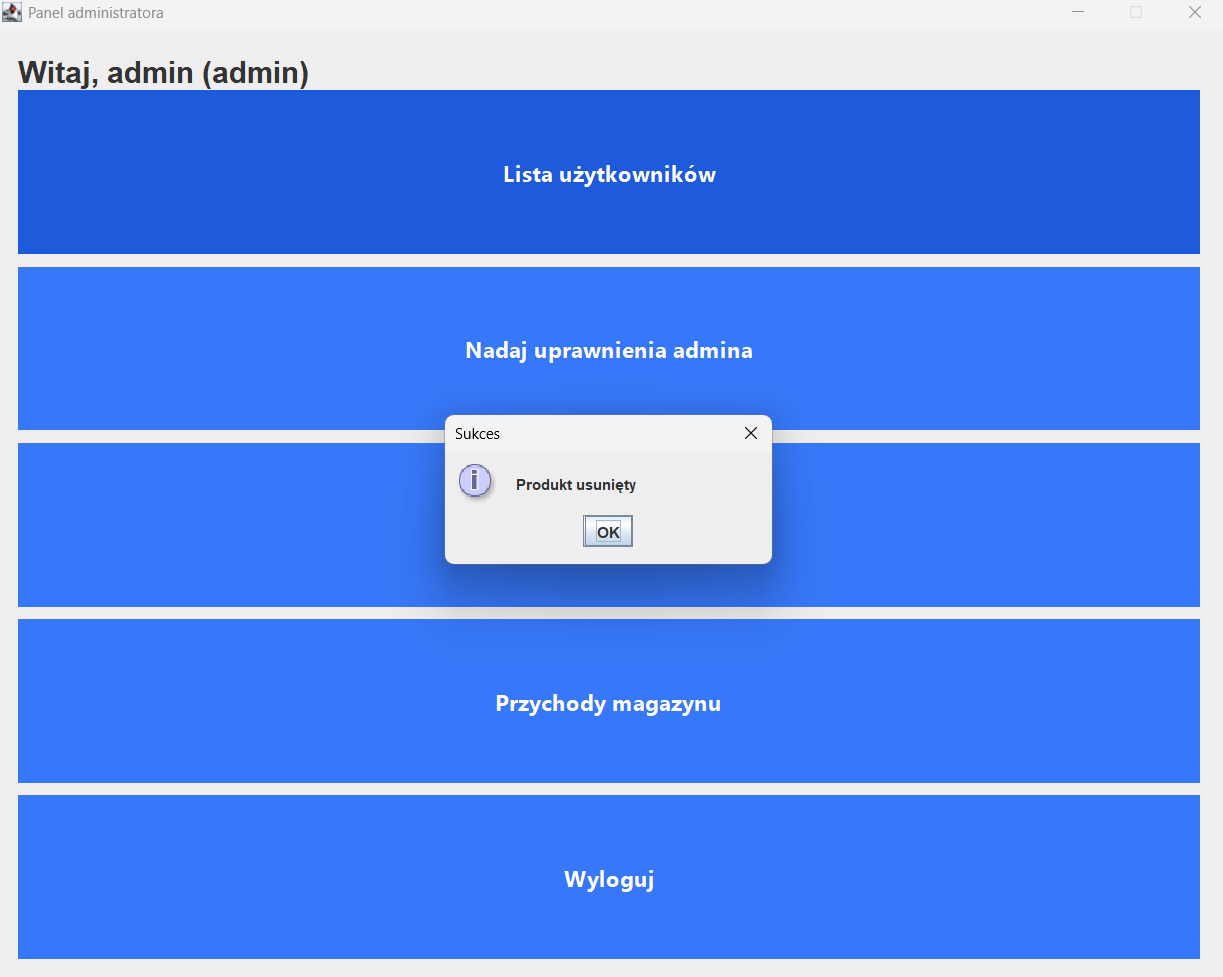
\includegraphics[width=.7\linewidth]{figures/PanelAdministratora2.png}\
    \caption{PanelAdministratora2.\label{PanelAdministratora2}}
\end{figure}
\clearpage
\subsection{Nadaj uprawnienia admina}
\label{subsec:Nadaj uprawnienia admina}
Po kliknięciu Nadaj uprawnienia admina wyświetla się takie okno 
\begin{figure}[H]
    \centering
    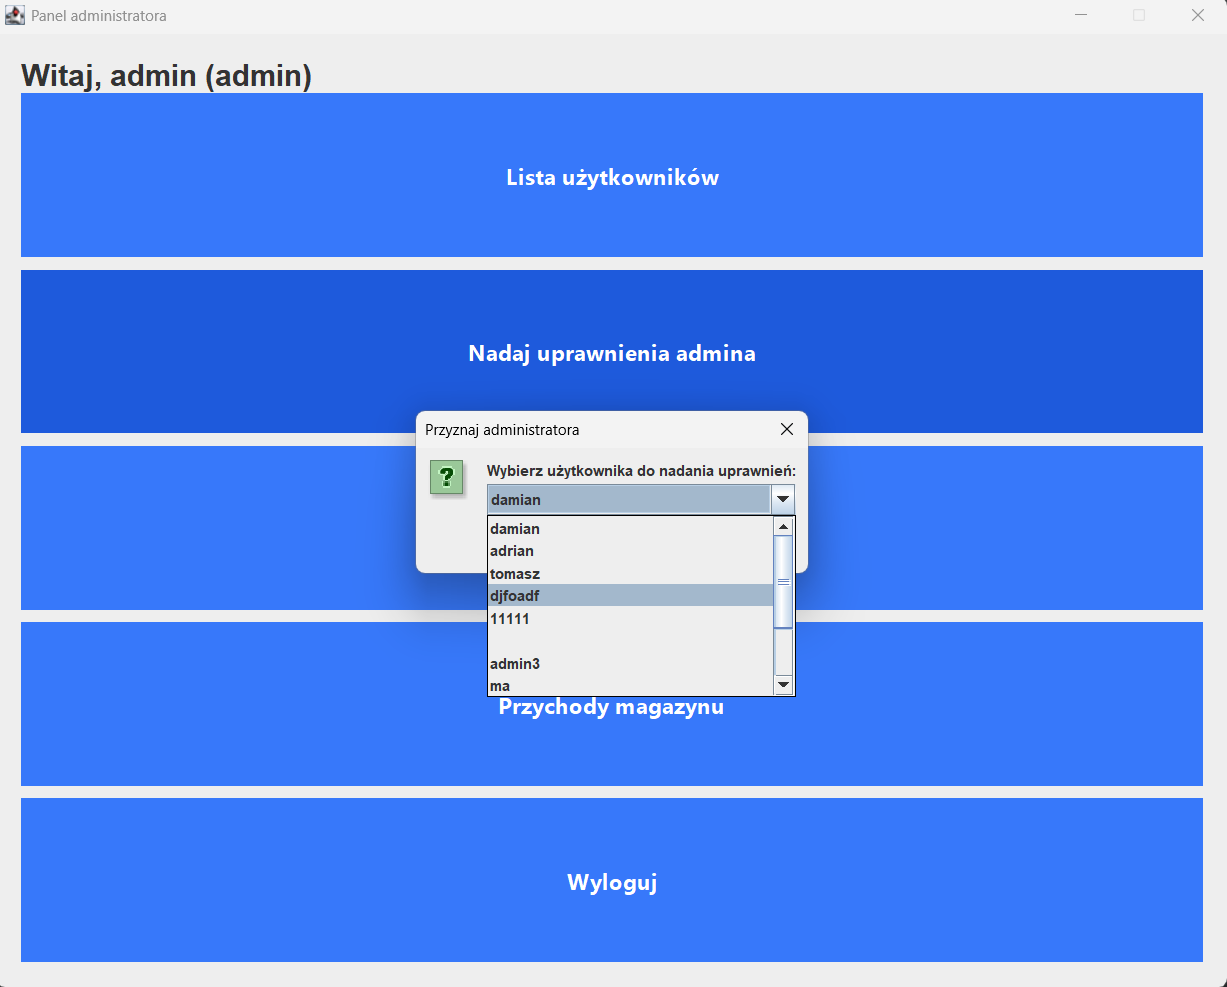
\includegraphics[width=.7\linewidth]{figures/PanelAdministratora3.png}\
    \caption{PanelAdministratora3.\label{PanelAdministratora3}}
\end{figure}
a po tym wyświetla komunikat:
\begin{figure}[H]
    \centering
    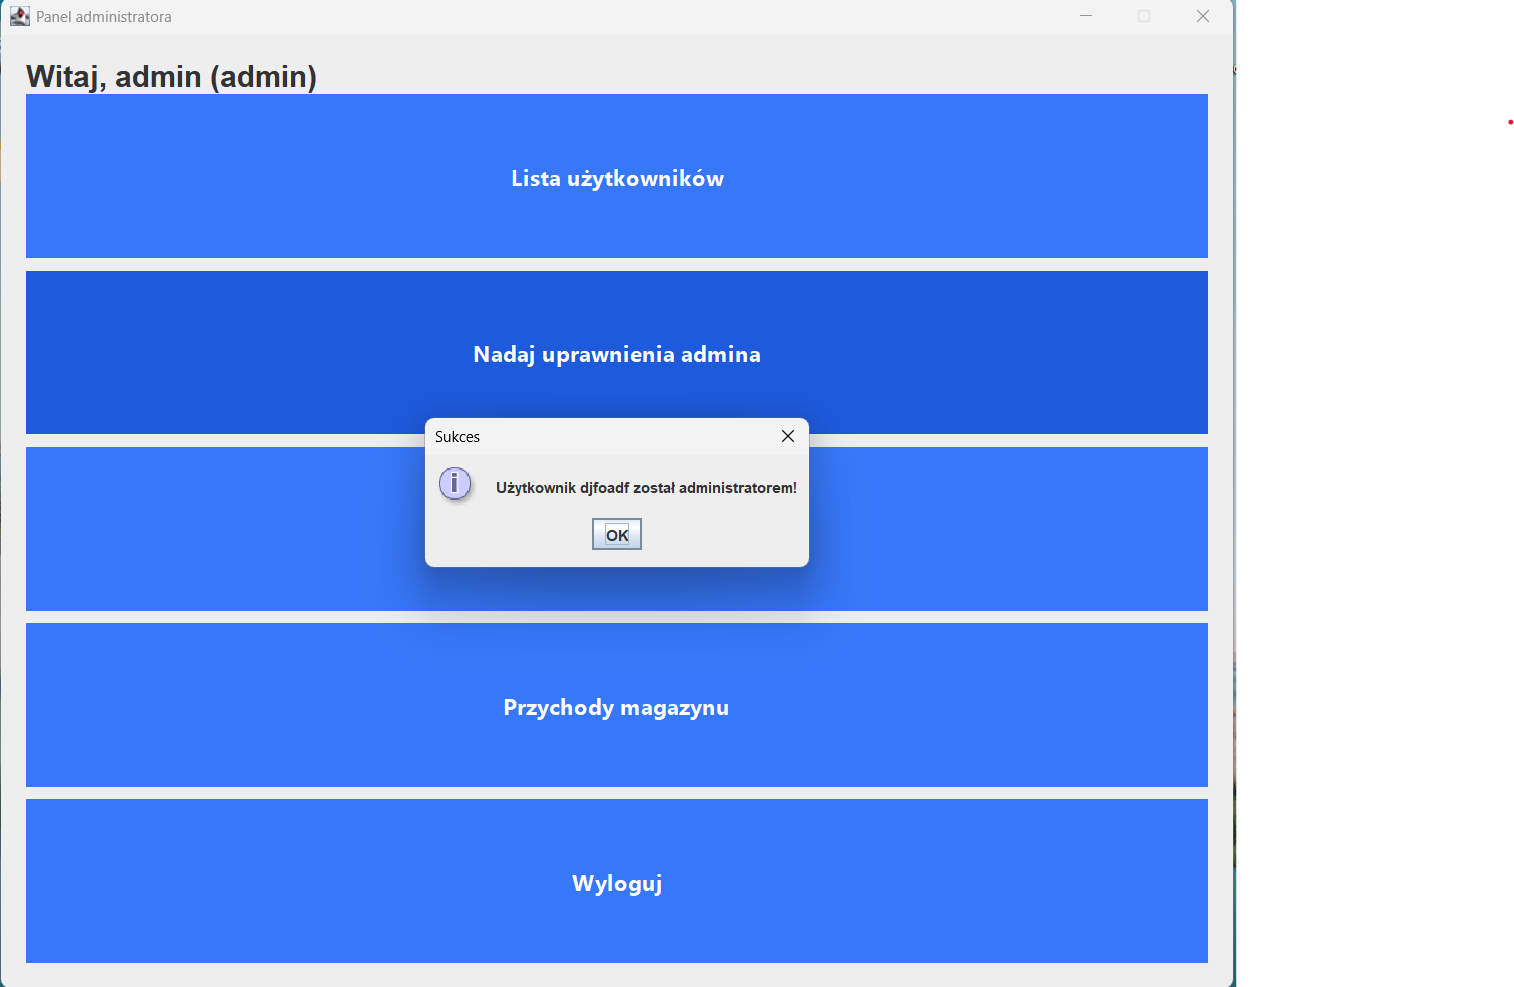
\includegraphics[width=.7\linewidth]{figures/PanelAdministratora5.png}\
    \caption{PanelAdministratora5.\label{PanelAdministratora5}}
\end{figure}
\clearpage
\subsection{Przekroczenia czasu}
\label{subsec:Przekroczenia czasu}
Gdy klikniemy Przekroczenia czasu wyświetli tabele z użytkownikami, którzy nie odebrali swojego materiału na czas
\begin{figure}[H]
    \centering
    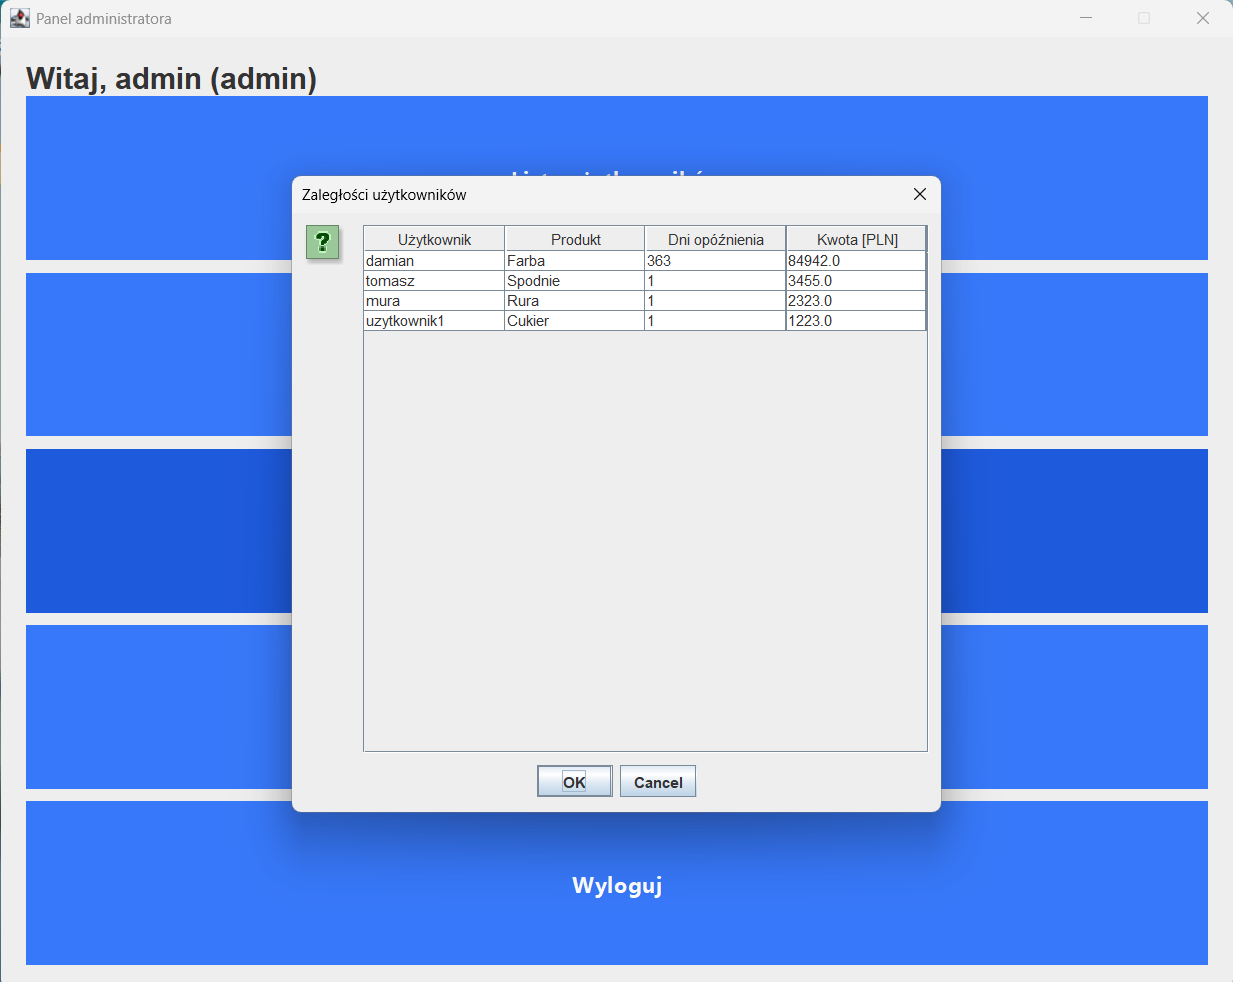
\includegraphics[width=.7\linewidth]{figures/PanelAdministratora6.png}\
    \caption{PanelAdministratora6.\label{PanelAdministratora6}}
\end{figure}
Jeśli zedytujemy coś w kolumnie kwota to usuwa uzytkownika z tego wiersza, w którym zedytowaliśmy kolumne kwota
\begin{figure}[H]
    \centering
    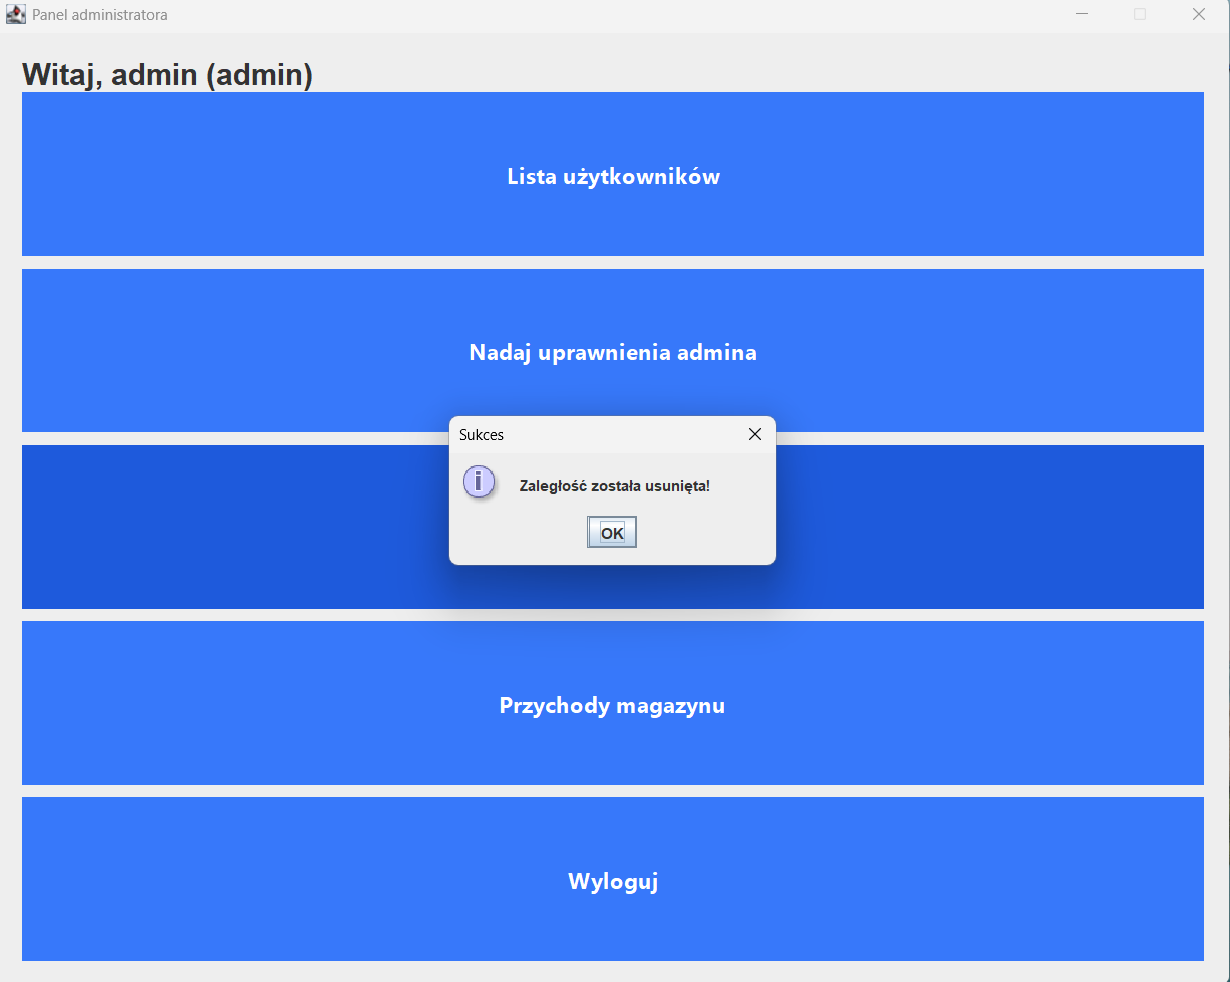
\includegraphics[width=.7\linewidth]{figures/PanelAdministratora7.png}\
    \caption{PanelAdministratora7.\label{PanelAdministratora7}}
\end{figure}
\clearpage
\subsection{Przychody magazynu}
\label{subsec:Przychody magazynu}
Wyświetla tabele z przychodami
\begin{figure}[H]
    \centering
    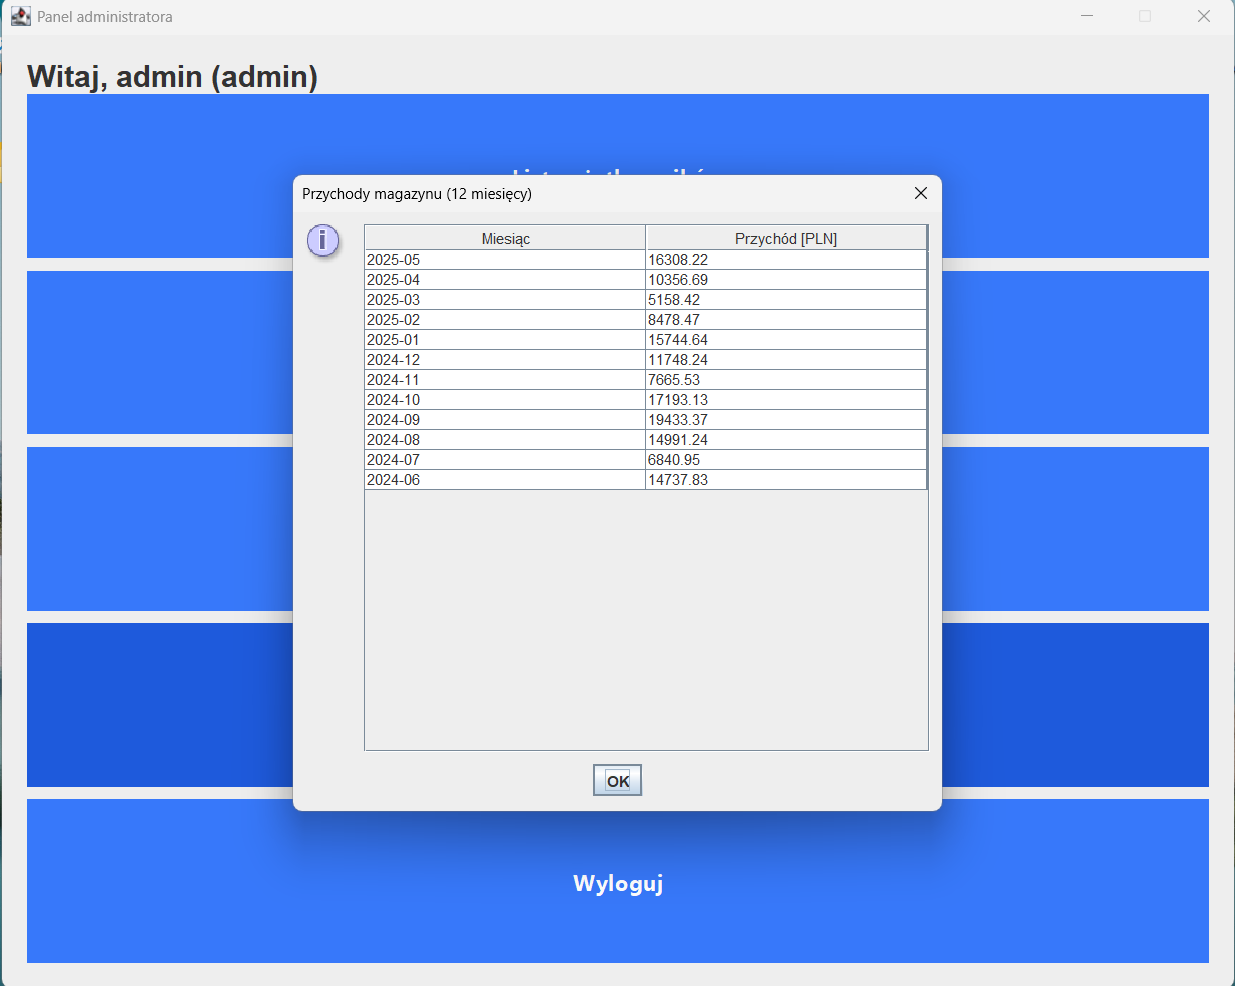
\includegraphics[width=.7\linewidth]{figures/PanelAdministratora8.png}\
    \caption{PanelAdministratora8.\label{PanelAdministratora8}}
\end{figure}
\clearpage
\subsection{Wyloguj}
\label{subsec:Wyloguj}
Po kliknięciu przycisku Wyloguj wyświetli się komunikat:
\begin{figure}[H]
    \centering
    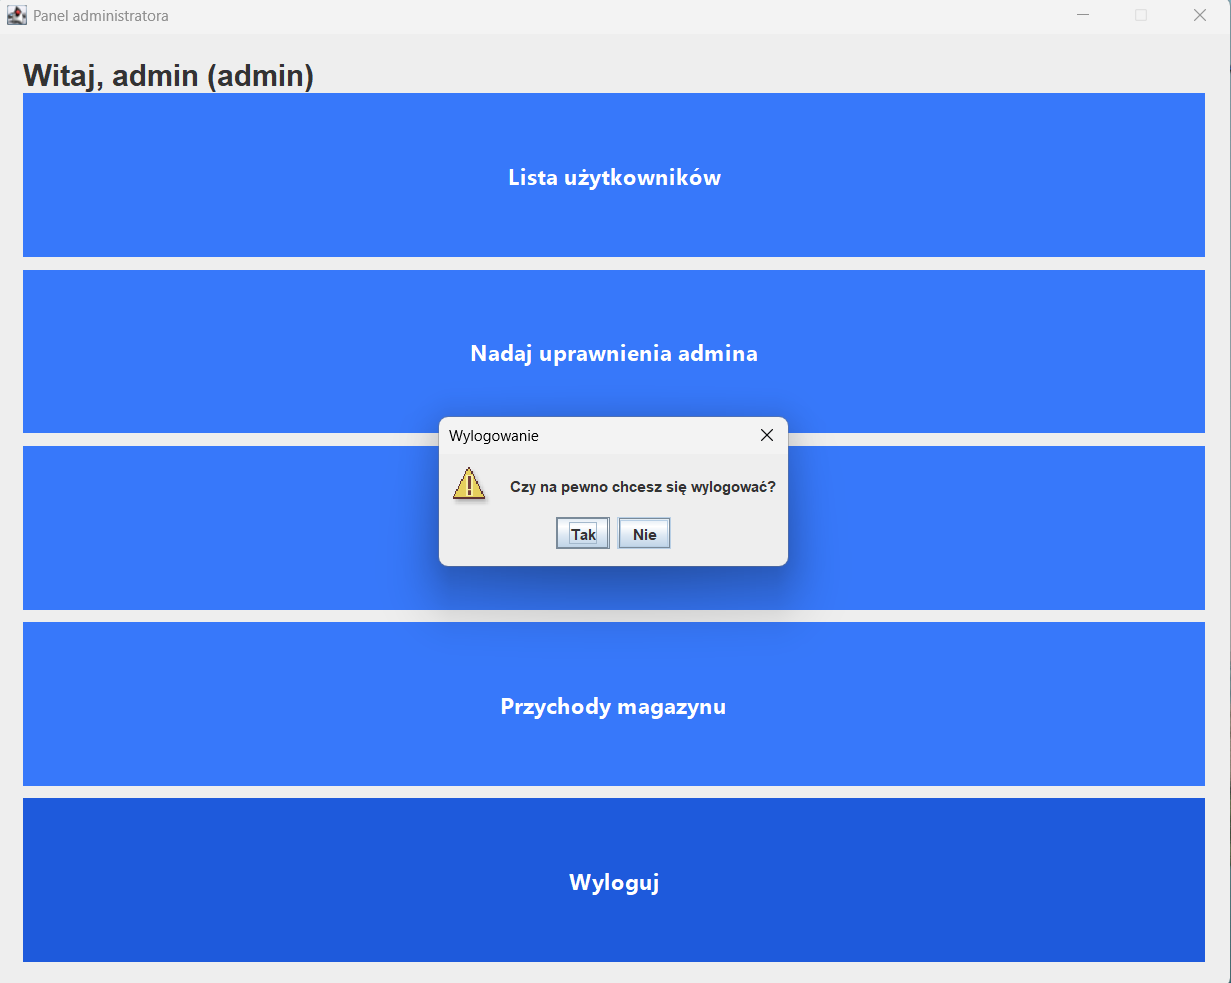
\includegraphics[width=.7\linewidth]{figures/PanelAdministratora9.png}\
    \caption{PanelAdministratora9.\label{PanelAdministratora9}}
\end{figure}